\documentclass[12pt, twoside]{report}
\setcounter{secnumdepth}{3}

\usepackage[utf8]{inputenc}
\usepackage[a4paper, width=150mm, top=25mm, bottom=25mm, bindingoffset=6mm]{geometry}

% formatting the header and the footer of the document
\usepackage{fancyhdr}
\pagestyle{fancy}
\fancyhead{}
\fancyhead[RO, LE]{Parallel Programming on Embedded Multicore System ESP32}
\fancyfoot{}
\fancyfoot[LE, RO]{\thepage}
\fancyfoot[LO, CE]{Chapter \thechapter}
\fancyfoot[CO, RE]{UPT Timișoara}
\renewcommand{\headrulewidth}{0.4pt}
\renewcommand{\footrulewidth}{0.4pt}

% including graphics, e.g. images
\usepackage{graphicx}
\graphicspath{{images/}}

% adding references system
% note: for linux (gummi), it was necessary to install the following packages:
%		- biber, biblatex, texlive-bibtex-extra, latexmk
%		=> in gummi: Edit->Preferences->Compilation->latexmk
\usepackage{biblatex}
\addbibresource{references.bib}

\usepackage{fancyref}
\usepackage{amsmath}
%\usepackage{mathtools}

\newcommand\vertarrowbox[3][6ex]{%
	\begin{array}[t]{@{}c@{}} #2 \\
		\left\uparrow\vcenter{\hrule height #1}\right.\kern-\nulldelimiterspace\\
		\makebox[0pt]{\scriptsize#3}
	\end{array}%
}

\title{
	{Parallel Programming on Embedded Multicore System ESP32\bigskip}\\
	{\large Universitatea Politehnica Timișoara\bigskip\bigskip}\\
	{
\includegraphics[width=50mm,scale=0.5]{upt_logo.png}}
}
\author{ Marian Belean\\ Franz Joseph Pal }
\date{ WS2019/2020 \\ \today}

\begin{document}

\maketitle

\pagenumbering{roman}

\chapter*{Abstract}
The following documentation will focus on the principles of parallel programming in general and the mathematical background. In addition to the different parallel programming architectures, the various models for their implementation are also discussed. Moreover, in this thesis the prerequisites for mathematical calculation models, which are suitable for Parallel Programming, are elaborated.\newline\newline
For a practical example, the ESP32 microcontroller was chosen, an embedded multicore system. After a brief introduction to the hardware itself, further details of the project structure and the development of the application will be presented. Therefore, a short example will be explained to focus on the basics of parallel programming.\newline\newline
Finally, the aim of the project and the documentation is an automatic benchmark setup and a webfrontend result overview for visualization purposes, which will be discussed in more detail in the conclusion. 

\chapter*{}
\centerline{\Large \textsf{\textbf{Declaration}}} \label{Declaration}%\\
\vspace*{2ex}
%
I hereby certify that I have done the final thesis on my own, that I have completely and accurately stated all the aids I have used and identified everything individually, which was taken from the work of others unchanged or with modifications.\\
\\
{\itshape
The topic of the submitted work was jointly with
Mr. / Mrs. (...) (Bachelor and Master Thesis No. (...)).
}\\

\vspace*{4ex}
Timișoara, the \today \\

\vspace*{4ex} 
Signature:\\


\vspace{2cm}

%--------------------------------------------------------------
\section*{}
\centerline{\Large \textsf{\textbf{Non-disclosure notice}}} %\\
\vspace*{2ex}
	
This work contains confidential information. In spite of the anonymous presentation of the researched organisations, readers might conclude their identity. Therefore copying, quoting or publishing is not allowed without my explicit authorisation. Furthermore, disclosure of the information to anyone other than the examination board or lectors is not authorized.

%**************************************************************

\tableofcontents

\chapter{Introduction}\label{chap:introduction}
Multicore systems are becoming increasingly popular as part of digitization and Industry 4.0\footnote{ add.: https://www.epicor.com/en-ae/resource-center/articles/what-is-industry-4-0/} (German/EU) \parencite{internet5} \parencite[or][]{article13} - also known as smart manufacoring in the USA \parencite[see][p1]{article12} - and are playing an important role in data processing and process automation \parencite[see][p294]{inproceedings3} \parencite[or][p1]{article11}. On the other hand, in addition to efficiency in energy consumption, performance in terms of computation time \parencite[see][p294]{inproceedings3} is required in almost every application field of multicore systems.

In fact, multicore hardware is not only exspecially for smart manufactoring. Nowerdays in almost every smart application like smart phones\footnote{ e.g. ARM based processors for mobile phones like https://www.arm.com/solutions/mobile-computing/smartphones}, wearables\footnote{ add. information on ARM based solutions and the current trend in wearables: https://www.arm.com/solutions/wearables} or home automation we can find multicore embedded hardware platforms, which garantued high performance \parencite[see][p7]{article15}, network connectivity, security and reliability \parencite[see][p5]{article16}. This field of application is also known as Internet of Things (IoT)\footnote{ for additional information about Internet of Things, please see \parencite[][]{article17}}.

Especially for embedded systems mathematical models as well as numerical solutions, which can be executed both simply and parallel, are suitable. The question arises to what extent parallel execution of different sub-tasks to calculate a problem \parencite[see][p4]{article14} increases the desired cost factor in terms of energy consumption \parencite[see][chapter 3]{inproceedings4} and computational efficiency \parencite[see][p4 Figure 3]{article14}.

\pagenumbering{arabic}

\chapter{Overview}\label{chap:overview}
\section{Problem definition}

Compared to single-core execution of tasks, multi-core embedded hardware platforms like the ESP32\footnote{add. information: https://www.espressif.com/en/products/hardware/socs} provide the ability to develop advanced parallel computing software applications to reduce execution time and power consumption.

On the one hand, a major problem is choosing the right hardware platform to meet the cost and size factor, and moreover, whether a single-core or multi-core calculation is required. Therefore, context switching time, power consumption and total execution time must be included in the evaluation.

In order to develop an optimal solution, the hardware platform must be included in addition to the mathematical model of the problem itself. So in this case, suitable prerequisites and characteristics can be worked out in order to make an evaluation of "Parallel Computation Tasks on Embedded Multicore Systems" possible.

\section{Objective of the documentation}

The main goal of this documentation is to focus on the current parallel programming techniques, depending on the execution time in general and the required mathematical model. For this purpose, an application which can compute different sections of the Mandelbrot fractal \parencite[see][p11]{article18} will be developed to compare single core and multi-core calculations. Before the practical implementation, an investigation based on parallel architectures and programming models will be conducted.

The elaboration is diveded into three different chapters: In the first chapter, the results of the general research are presented [see \fref{chap:parallelprg}]. After that, the second chapter is pointing out the practical implemenation of the developed application on the ESP32 [see \fref{chap:documentation}]. In the end, the results including the webforntend and the automatic benchmark setup [see \fref{chap:conclusion}] will be discussed.

\chapter{Parallel Programming in General}\label{chap:parallelprg}
\section{Basic Concept}

\underline{Amdahl's law} \parencite{book6}:

\begin{figure}[h!]\centering
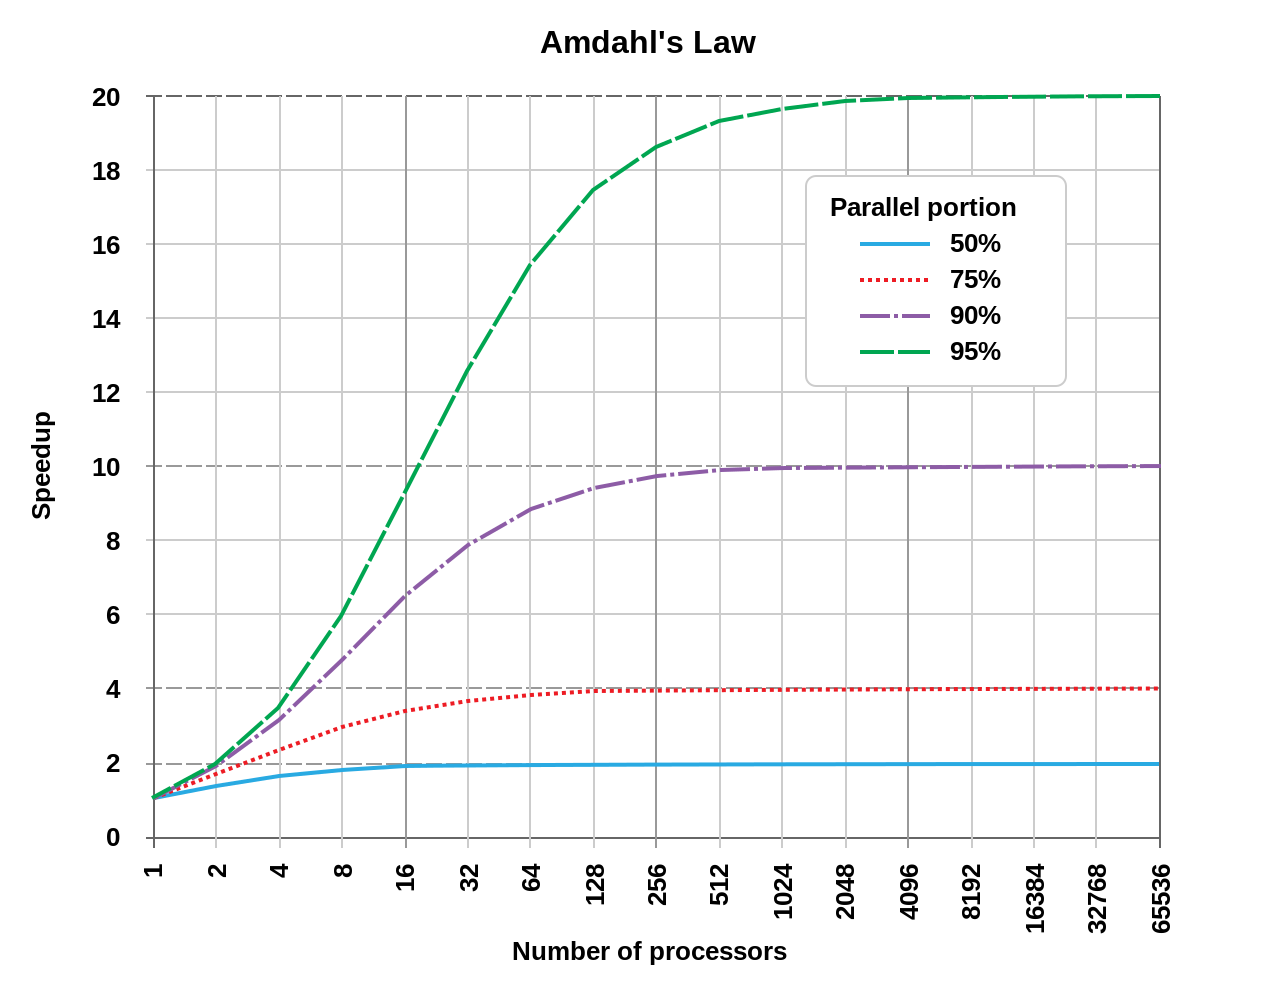
\includegraphics[scale=0.8]{amdahls-law.png}
\caption{
...
}
\label{fig:admLaw}
\end{figure}

\begin{itemize}
\item “the contention that the organization of a single computer has reached its limits and that
truly significant advances can be made only by interconnection of a multiplicity of computers” \parencite[see][p80]{inbook1}; can be transferd on single and multi-core processors or even on multithreading, but in fact, like Amdahl claimed too, adressing hardware, and nowerdays switching context time was not considered here!
Valiant noted in 1990, “no substantial impediments to general-purpose parallel
computation” exist \parencite[see][p85]{inbook1}, though there are limits, as shown \parencite[seein Sec. 10][p85]{inbook1}.

\newpage

\item “the fraction of the computational load... associated with data management housekeeping ... accounts for 40\% of the executed instructions”, "this overhead appears to be sequential so that it is unlikely to be amenable to parallel processing techniques” \parencite[see][p80]{inbook1}; amount of overhead (data management and adressing based on hardware restricitons), which can not be parallelized and reduces the factor of speed increase after parallelization. According to Amdahl, this factor can be reduced, but not with "parallel processing techniques", probably with more precisely and efficent hardware.
\item a resisting "upper limit on speedup [exists] and therefore, apart from the sequential fraction (the so called non parallelizabled overhead), the remaining computations are perfectly parallelizable" \parencite[see][p81]{inbook1}
\item the law in general: Let t\textsubscript{1} be the time taken by one processor solving a computational problem and t\textsubscript{p} be the time taken by p processors solving the same problem. Finally let us denote the supposed inherently sequential fraction of instructions by f. Then, according to Amdahl, t\textsubscript{p} = t\textsubscript{1} (f+(1-f)/p) and the speedup obtainable by p processors can be expressed as:

	
\[ \frac{t_1}{t_p} = \frac{1}{f + (1 - f) / p)} \]
\end{itemize}

\newpage

\subsection{Principles of Parallel Computing}

\textbf{Emphasises design}:
Amdahl's law highlights the pitfalls of looking for
sticking-plaster speed-ups in serial programs –
design for concurrency \parencite[see][p4]{article6}
\\\\\textbf{Aim of concurrency and their effects} on program structure or implementation \parencite[see][p5]{article6}:
\begin{itemize}
  \item \underline{Flexibility}: Environments will be more heterogeneous.
  \item \underline{Efficiency}:	parallel for a speed-up purposes, more pitfalls (memory latency, thread overheads etc.)
  \item \underline{Simplicity}:	Parallel codes will be more complicated. All the more reason to strive for maintainable, understandable programs.
\end{itemize}

\newpage

\section{Definition of parallel mathematical computations}


...\newpage

\section{Parallel Computer Architecture}

...\parencite[see][p9]{book1} \\
...examples of parallelism \parencite[see][p11]{book1}

\subsection{Flynn's Taxonomy of Parallel Architectures}

...\parencite[see][p5]{internet1}\\
...\parencite[see][p13]{book1}\\
...\parencite[see][p4]{book5}\\
...\parencite[see][p2]{book6}\\

\subsection{Thread Level Parallism}

...\parencite[see][p24]{book1}

\section{Parallel Programming Models}

\textbf{Steps to evaluate a proper parallel design} \parencite[see][p6]{article6}:
\begin{enumerate}
	\item Finding Concurrency
	\item Algorithm Structure
	\item Supporting Structures
	\item Implementation Mechanisms
\end{enumerate}

\newpage

\subsection{Classification of Parallel Programming Models}

\subsubsection{Process Interaction}

...\parencite[see][p4]{internet1}

\subsubsection{Problem decomposition}

...\parencite[see][p105 ff.]{book1}

\chapter{Project documentation}\label{chap:documentation}
\section{Simple mathematical computation example for Parallel Programming} \label{chap:simpleMathCompParallel}

Before going into detail about the Mandelbrot computation, we will discuss as a first example a basic computation as already mentioned in Chapter \ref{chap:mathComp}. The reason we are doing that is to reduce complexity and to point out the main parts, we will need for the Mandelbrot computation as well. In formula \ref{formula:scalarProdSeq}, we have pointed out that the computation of a simple scalar product of two vectors with the same dimension \textit{N} can be split into several sub task \textit{p}. Our modified version is based on two sums. The outer one will iterate [index \textit{i}, see formula \ref{formula:twoLoopSum}] from zero to an upper limit \textit{N\textsubscript{1}} and sum up the result from the inner sum, which will perform a sum from 0 to \textit{N\textsubscript{2}} [index \textit{j}, see formula \ref{formula:twoLoopSum}] over a multiplication of \textit{i} and \textit{j}. The following formula represent the announced mathematical problem:

\begin{align} \label{formula:twoLoopSum}
\begin{aligned}
s &= \sum_{i = 0}^{N_1} \left( \sum_{j = 0}^{N_2} \left(i \cdot j\right) \right)
\end{aligned}
\end{align}
\

To process the problem in parallel, it is only possible to seperate the outer sum into sub sums regarding to formula \ref{formula:twoLoopSumParallel}.

\begin{align} \label{formula:twoLoopSumParallel}
\begin{aligned}
s &= \sum_{i = 0}^{N_1} \left( \sum_{j = 0}^{N_2} \left(i \cdot j\right) \right)
\\ &=  \underbrace{ 
	\sum_{i = 0}^{\frac{N_1}{2} - 1} \left( \sum_{j = 0}^{N_2} \left(i \cdot j\right) \right)
}_\text{p\textsubscript{0}} \qquad \vertarrowbox{+}{process communication} \qquad \underbrace{  
	\sum_{i = \frac{N_1}{2}}^{N_1} \left( \sum_{j = 0}^{N_2} \left(i \cdot j\right) \right)
}_\text{p\textsubscript{1}}
\end{aligned}
\end{align}
\

For collecting the part results from the parallel computed sums, some sort of process communication [see formula \ref{formula:twoLoopSumParallel}] between the threads is necessary, more then, its impossible without it. 

\newpage

But actually, this is the task, we have to take care about most. Otherwise we will run into race conditions while addressing same resources or even blocking methods, which will result in wrong execution time measurements.

As mentioned in Chapter \ref{chap:parPrgModels}, a common solution to communicate between threads running on different cores is using the \textbf{Message Passing Model} [for more details, see Chapter \ref{subsection:processInteraction}]. Our aim is to pass the computed part results to a main ``actor'', which will collect the part sums to calculate the final result. Furthermore, for bench-marking this setup, we will implement a time measurement mechanism to evaluate the decrease of execution time running the computation on one or both cores. 

Formula \ref{formula:twoLoopSumParallel} is theoretically not limited to the dedicated number of cores, which the hardware platform offers. Each core can handle multiple threads, but in this case, we would leave real time parallelism, because each core now has to handle multiple threads by the scheduler. Every thread on each core will be given some execution time between switching the context to the next one. An overall speedup is not guaranteed with this method.   

\newpage

\subsection{UML diagram}

This little mathematical example can be found on our GitHub repository \parencite{internet12} and is basically split into three parts. The main \textit{*.ino} file, and two classes, the \textit{Computation.h} and the \textit{Benchmark.h}. 

\begin{figure}[htbp]
	\centering
	\begin{subfigure}{.5\textwidth}
		\centerline{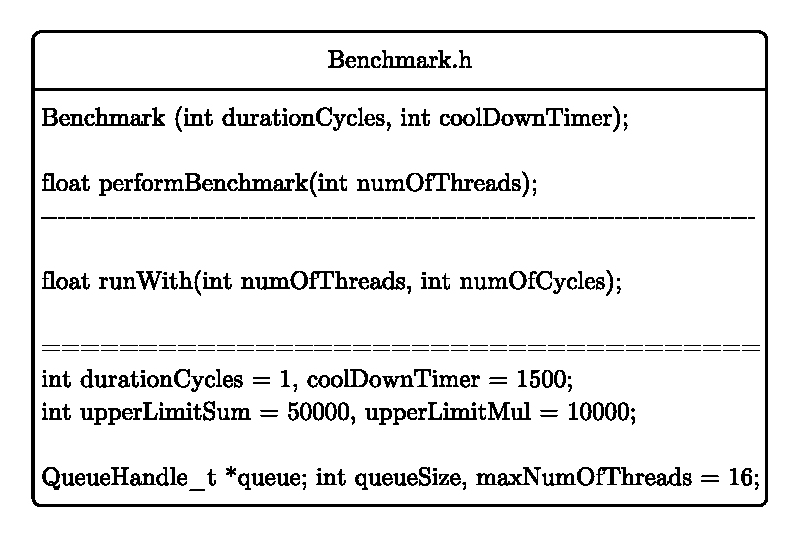
\includegraphics[width=1\linewidth]{images/Benchmark-UML.pdf}}
		\caption{ UML diagram Benchmark.h class }
		\label{fig:benchUML}
	\end{subfigure}%
	\begin{subfigure}{.5\textwidth}
		\centerline{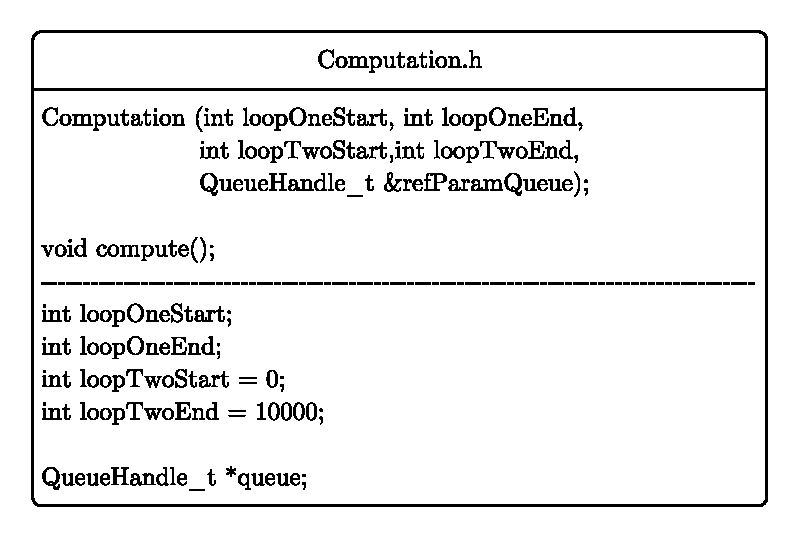
\includegraphics[width=1\linewidth]{images/Computation-UML.pdf}}
		\caption{ UML diagram Computation.h class }
		\label{fig:compUML}
	\end{subfigure}
	\caption{Overview over both main implementations regarding Chapter \ref{chap:simpleMathCompParallel}}
	\label{fig:umlDiagrBasicExample}
\end{figure}

\subsection{Implementation}

The \textit{Benchmark.h} class has several functions to set the necessary parameters to start a benchmark like mentioned at the end of Chapter \ref{chap:simpleMathCompParallel}. The computational problem discussed in formula \ref{formula:twoLoopSumParallel} is implemented in \textit{Computation.h} class regarding to the following function.

\begin{lstlisting}
void Computation::compute() {
	long count = 0;
	
	for (int i = getStartOne(); i < getEndOne(); i++) {
		for (int j = getStartTwo(); j < getEndTwo(); j++) {
			count += i * j;
		}
	}
	
	/* process communication */
	
	xQueueSend(*queue, &count, portMAX_DELAY);
}
\end{lstlisting}

It is obvious, based on simple mathematical rules, that the outer sum, which is implemented through the outer for-loop, is divisible by limiting the thresholds, the inner sum unfortunately isn't. So for each part sum it's necessary to calculate the limits, on which each task has to compute their part sum results \parencite[see][Benchmark.h, line 94 ff.]{internet12}.

\newpage

\noindent To start the benchmark, we have to include the \textit{Benchmark.h} header file, and create an object of it. In the constructor, it is necessary to specify the amount of duration's per cycle (for averaging the result), the time to wait until the next benchmark execution will be started and the queue size.

\begin{lstlisting}
Benchmark bench(1, 1500, 8);

for (int i = 0; i < numOfRunningThreads; ++i) {
	results[i] = new float(bench.performBenchmark(i + 1));
}
\end{lstlisting}

The queue size represents the maximum number of threads, which can be executed in parallel, because each thread has to return the result to the main thread; this is done by a ESP32 specific \textit{QueueHandle\_t} message passing model between tasks. Keep in mind, that this has an major effect of the available stack or heap size, and of course on the maximum amount of created threads [for more information about the \textit{QueueHandle\_t} thread communication, see \textit{Benchmark.h} line 99 ff.].\\

\noindent So let's become more concretely: We start for our outer for-loop [see formula \ref{formula:twoLoopSumParallel}] with \textit{i} from 0 to \textit{N\textsubscript{1}} equals 50000. Our inner for-loop has it's limit at \textit{N\textsubscript{2}} = 10000. If we now want to split this computation into four separated tasks, two on core 0 (t\textsubscript{1}, t\textsubscript{2}) and two on core 1 (t\textsubscript{3}, t\textsubscript{4}). The new limits for the part sums can be calculated using the formula below:

\begin{lstlisting}[label={code:calcLimits}]
float Benchmark::runWith(int numOfThreads) {
	...
	
	for (int k = 0; k < numOfThreads; k++) {
	
		/* outer sum i = 0 ... N1 */
		int lowLimSum = (50000 / numOfThreads) * k;
		int uppLimSum = (50000 / numOfThreads) * (k + 1);
		
		/* inner sum j = 0 ... N2 */
		int uppLimMul = 10000;
		
		if(50000 % numOfThreads != 0 && k == numOfThreads - 1) {
			uppLimSum += (50000 % numOfThreads);
		}
	
		c[k] = new Computation(	lowLimSum, uppLimSum, 
								0, uppLimMul, *queue );
	
		...
	}
}
\end{lstlisting}

Our new limits for the part sums are now the ones mentioned in formula \ref{formula:partSums} and are summed up in table \ref{table:partSumLimits}.

\newpage

\begin{align} \label{formula:partSums}
\begin{aligned}
	s_a &= \sum_{i = 0}^{12499} \left( \sum_{j = 0}^{10000} \left(i \cdot j\right) \right) &, 
	s_b &= \sum_{i = 12500}^{24999} \left( \sum_{j = 0}^{10000} \left(i \cdot j\right) \right) \\
	s_c &= \sum_{i = 25000}^{37499} \left( \sum_{j = 0}^{10000} \left(i \cdot j\right) \right) &, 
	s_d &= \sum_{i = 37500}^{50000} \left( \sum_{j = 0}^{10000} \left(i \cdot j\right) \right)
\end{aligned}
\end{align}\\

\noindent The implementation of the part sum limits is a little bit different to the mathematical description regarding formula \ref{formula:partSums}, because we are using for-loops and to determine the end of the sum, we are using a ``\textit{less than}'' operator. So therefore the threshold limits can be found in the table below.

\renewcommand{\arraystretch}{1.5}

\begin{table}[h!]
	\centering
	\begin{tabular}{ | m{3cm} | m{3cm} | m{3cm} | m{3cm} |  }
		\hline
		\multicolumn{4}{|c|}{Part sum limits} \\
		\hline
		Thread t\textsubscript{1} on core p\textsubscript{0} & 
		Thread t\textsubscript{2} on core p\textsubscript{1} &
		Thread t\textsubscript{3} on core p\textsubscript{0} &
		Thread t\textsubscript{4} on core p\textsubscript{1} \\
		\hline
		i = 0 & i = 12500 & i = 25000 & i = 37500 \\
		\vdots & \vdots & \vdots & \vdots \\
		i \textless 12500 & i \textless 25000 & i \textless 37500 & i \textless 50000 \\
		\hline
	\end{tabular}
	\caption{ Overview over the separated for-loop sum limits for four threads }
	\label{table:partSumLimits}
\end{table}

But what happened if we have an odd number of threads? Well in this case, the \textit{Benchmark.h} class handle the issue, too. The upper limit will be divided into even part sum limits and for the last thread, the upper limit consists of the even upper limit plus the rest until he reaches 50000. This is done by an if clause and a ``\textit{modulo}'' operator [see \ref{code:calcLimits}]. After determine the necessary limits and amount of threads, we are now able to create the tasks and assign them to a dedicated core. As mentioned before, real time parallelism can only be achieved by using the exact or less number of cores. 

\begin{lstlisting}[label={code:createThreads}]
for (int j = 0; j < numOfThreads; j++) {
	...
	
	c[j] = new Computation(	lowLimSum, uppLimSum, 
							0, uppLimMul, *queue );
	
	xTaskCreatePinnedToCore(
		producerTask,
		(j+1)%2 ==  0 ? "calcTask0" : "calcTask1",
		sizeof(c[j]) * 32 * 8,
		c[j],
		0,
		NULL,
		(j+1)%2 );
}
\end{lstlisting}  

\newpage

\subsection{Implementation of the Message Passing Model}

\begin{figure}[htbp]
	\centerline{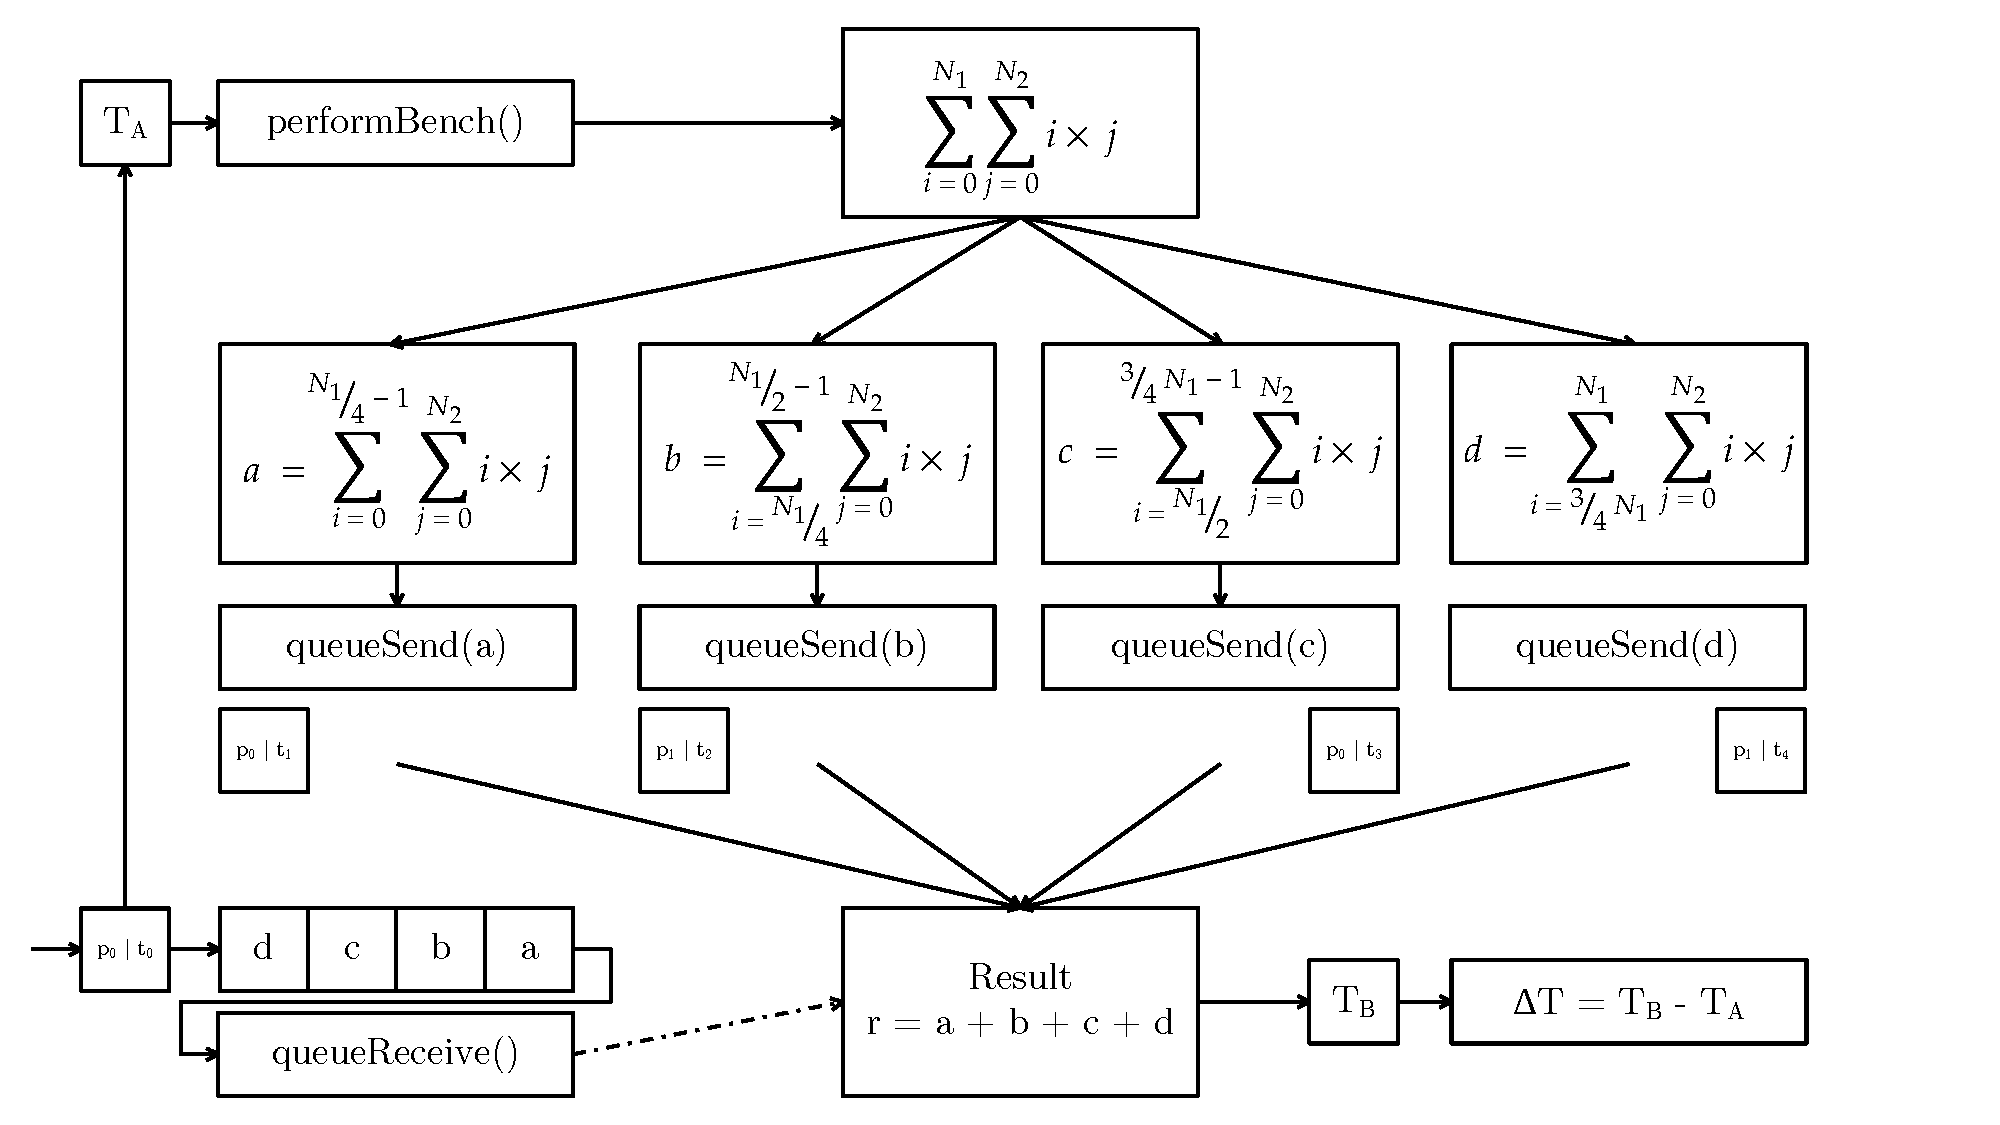
\includegraphics[width=1.1\linewidth]{images/Split-Sum-Message-Passing.pdf}}
	\caption{ Overview of the benchmark setup for the Computation example }
	\label{fig:splitSumOverview}
\end{figure}

\noindent If we now want to compare results regarding running the Computation on different cores, or even with multiple threads, we have to implement a time measurement functionality. This is done by the \textit{Benchmark.h} class. Before starting a Computation, we are saving a time stamp, and after all part results are collected, we take another one. Basically the time needed performing the tasks is the delta time between those two time stamps. But this lead into one main problem: How can we determine we collected all results, because this is an asynchronous event. 

Now our \textit{QueueHandle\_t} object will help once again. If we send back our results, the receiver will wait as long as a new object is pushed into the queue. As far as we know, we have to receive the passed \textit{numOfThreads} amount of part results. Combining these both examples will result into the following implementation:

\begin{lstlisting}[label={code:queueReceive}]
for (int k = 0; k < numOfThreads; k++) {
	long partResult;
	
	/* process communication -> receiving part results */
	xQueueReceive(*queue, &partResult, portMAX_DELAY);
	
	result += partResult;
}
\end{lstlisting}  

The last parameter for the \textit{xQueueReceive} function defines how long the receiver should wait until he should give up waiting. This is now set to a macro defining to wait as long as possible or until the queue is full. The passed reference will be used to add it to the result sum.

\newpage

\section{Introduction to the Mandelbrot fractal} \label{chap:mandelbrotIntroduction}
The Mandelbrot set is generated by iterations, which means to repeat a process over and over again. In mathematics this process is most often the application of a mathematical function.
For the Mandelbrot set, the functions involved are some of the simplest imaginable: they all are what is called quadratic polynomials and have the form 

\begin{align} \label{formula:mandelbrotFomrula}
	\begin{aligned}
		f(z) = z^2 + c
	\end{aligned}
\end{align}\\

or even described with

\begin{align} \label{formula:mandelbrotFomrula2}
	\begin{aligned}
		M = \left\lbrace \quad c \in C \quad | \quad lim_{n \rightarrow \infty} Z_n \neq \infty \quad \right\rbrace  
	\end{aligned}
\end{align}\\

where c is a constant number and M the complex series containing the values which are in the Mandelbrot set. Our main boundaries for the Mandelbrot set can be calculated as well, but we won't discuss this here. Let's say we take them for granted as shown in Figure \ref{fig:mandelbrotSet}. So what we have to specify now is the complex value \textit{c} in formula \ref{formula:mandelbrotFomrula}.

\begin{figure}[htbp]
	\centerline{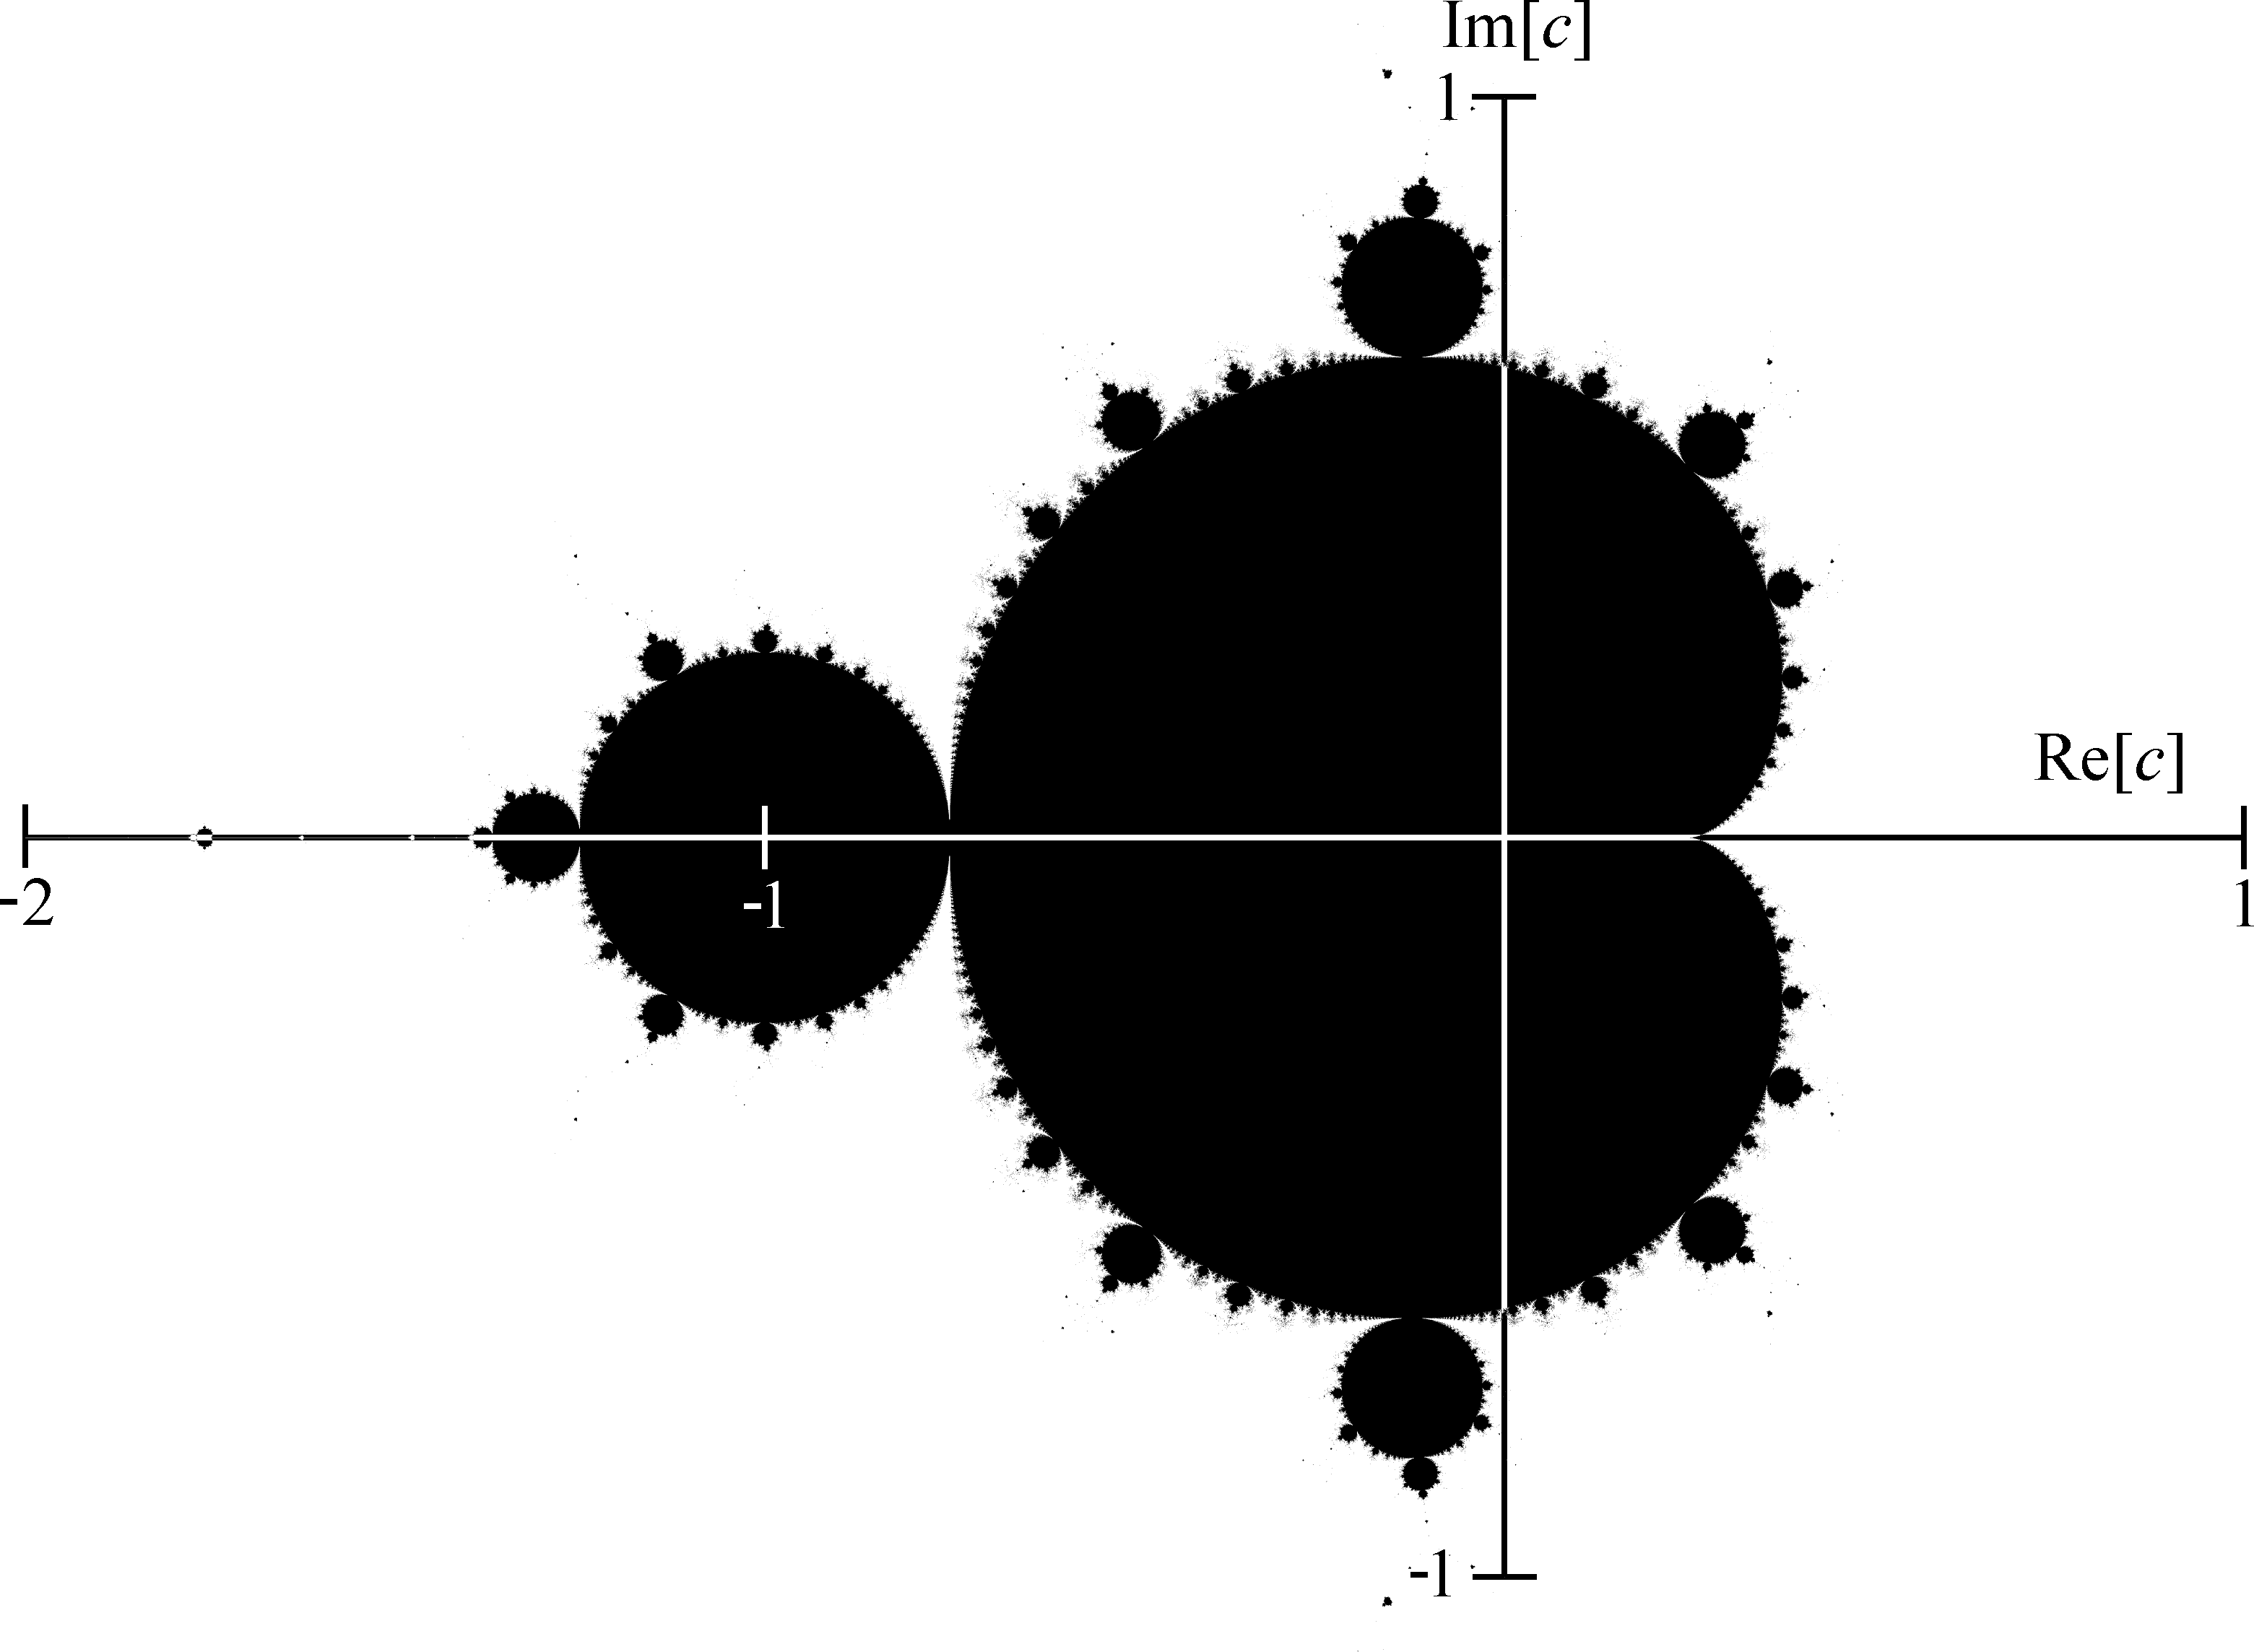
\includegraphics[width=0.9\linewidth]{images/Mandelset_hires.png}}
	\caption{ A mathematician's depiction of the Mandelbrot set M \parencite{internet14}. }
	\label{fig:mandelbrotSet}
\end{figure}  

\newpage

If we want to distinguish whether a point belongs to the Mandelbrot or not, we have to go through the mathematical description mentioned in formula \ref{formula:mandelbrotFomrula2}. We start with a chosen complex value \textit{c\textsubscript{0}} between our predefined boundaries, and pass this to formula \ref{formula:mandelbrotFomrula} as \textit{c}. The first result \textit{Z\textsubscript{0}} will be now the passed value \textit{c} (f(0) = \textit{c}), and can be recursively passed as \textit{z} again into the function to compute \textit{Z\textsubscript{1}}. Formula \ref{formula:mandelbrotFomrula} can therefore be also described as follow:

\begin{align} \label{formula:mandelbrotIteration}
	\begin{aligned}
		Z_0 \quad &= \quad c,\\
		Z_{n+1} &= \quad Z_n^2 + c\\
		\vdots
	\end{aligned}
\end{align}\\

\noindent If Z\textsubscript{n}, for \textit{c} as our complex value under test, now goes to $\infty$, \textit{c} doesn't belong to the Mandelbrot set \textit{M}, if not, this is a point of our complex series.

The definition [see formula \ref{formula:mandelbrotIteration}] in combination with formula \ref{formula:mandelbrotFomrula2} brings up two questions: Is it even possible to check whether the predefined complex value \textit{c} passed to the Mandelbrot set function goes to $\infty$, especially on a micro controller? And if we are able to reach $\infty$ somehow, our computed value will be very big, so how can we deal with that on limited hardware?

These questions are more or less related, and not very complicated to solve. If we take a closer look into the general definition of a complex value, it can be proofed that ``\textit{if the absolute value of Z ever gets bigger than 2, it will never return to a place closer than 2, but it will actually rapidly escape to infinity}'' \parencite{internet15}. In general that means we only have to check if the absolute value of our current \textit{Z\textsubscript{n}} goes bigger than two and therefore both problems are solved. But how often do we have to iterate through, to become more precisely, what is our threshold for \textit{n} in formula \ref{formula:mandelbrotFomrula2}?

Well, this can easily be shown if we calculate the Mandelbrot set for different maximal iterations for \textit{n} [see Figure \ref{fig:mandelbrotItertions}, \textit{n} starting from 0 to 40 in steps by 10].

\begin{figure}[htbp]
	\centerline{
\includegraphics[width=0.9\linewidth]{images/mandelbrot-iterations.png}}
	\caption{ Mandelbrot Set using different numbers of iterations.}
	\label{fig:mandelbrotItertions}
\end{figure}  

It is obvious, based on Figure \ref{fig:mandelbrotItertions}, that the number of iterations we go through during checking if the absolute value of the complex number under test is less than two, regarding to the image resolution, has no major effect after more than 30 iterations. The image we are calculating is ``\textit{not infinitely accurate}'', due to the fact that we are using pixel to plot the complex values. A considerable change in the image after a certain number of iterations \parencite{internet15} is not visible, therefore a larger number of iterations won't give us ``\textit{anything new to the image}'' \parencite{internet15}. 

\newpage

\subsection{The Mandelbrot set implementation} \label{subsection:mandelbrotCalc}

As we already know, the Mandelbrot set \textit{M} [see formula \ref{formula:mandelbrotFomrula2}] can be calculated defining our main Cartesian complex boundaries while looping through all the points and test whether the complex value \textit{c} belongs to the Mandelbrot set \textit{M} or not. So basically our computation function consists of a part defining our complex boundaries 

\begin{lstlisting}[label={code:mandelbrotBoundaries}]
	/* Cartesian 2D boundaries */
	double MinRe = -1.2;
	double MaxRe = 1.2;
	double MinIm = -1.2;
	double MaxIm = 1.2;
	
	/* to get the complex value of a pixel point P(x|y) */
	double Re_facor = (MaxRe - MinRe) / (width - 1);
	double Im_factor = (MaxIm - MinIm) / (height - 1);
	
	/* implementation of the mathematical limes */
	/* -> to infinite (in this case 34) */
	unsigned MaxIterations = 34;
\end{lstlisting}  

and how many iterations we want to go through, that meas how precisely we want to plot the image. After that, we have two for-loops going through all the pixel coordinates, which each has a corresponding complex value, to check whether they are in the Mandelbrot set or not \parencite{internet15}:

\begin{lstlisting}[label={code:mandelbrotForLoops}]
for (unsigned y = minY; y < maxY; ++y) {
	double c_im = MaxIm - y * Im_factor;

	for (unsigned x = minX; x < maxX; ++x) {
		double c_re = MinRe + x * Re_facor;

		double Z_re = c_re, Z_im = c_im;
		bool isInside = true;

		/* check if complex number Z belongs to M */
		for (unsigned n = 0; n < MaxIterations; ++n) {
			double Z_re2 = Z_re * Z_re, Z_im2 = Z_im * Z_im;

			if (Z_re2 + Z_im2 > 4) {
				isInside = false;
				break;
			}

			Z_im = 2 * Z_re * Z_im + c_im;
			Z_re = Z_re2 - Z_im2 + c_re;
		}
		
		/* draw pixel */
		if(isInside) { putpixel(x, y); }
	}
}
\end{lstlisting}

\newpage

\noindent In this case, we used a lot of simplifications to avoid complex mathematical functions, which require including specific libraries we probably won't have on our \textit{ESP32}. On of those are for example computing the absolute value of a complex number [see line 12, \ref{code:mandelbrotForLoops}]:

\begin{align} \label{formula:simplicityOne}
	\begin{aligned}
		abs(Z) \quad &= \quad \sqrt{Re\left\lbrace Z \right\rbrace^2 + Im\left\lbrace Z \right\rbrace^2} > 2\\
		Z^2 \quad &= \quad Re\left\lbrace Z \right\rbrace^2 + Im\left\lbrace Z \right\rbrace^2 > 4
	\end{aligned}
\end{align}\\ 

After we found a complex value which fulfills the above condition \textit{M}, we have to compute the next value regarding formula \ref{formula:mandelbrotFomrula}. The addition of two complex numbers is quite simple. However, complex number multiplication like \textit{z\textsuperscript{2}} in comparison to the addition is not that easy. But this process can  be simplified as well.

\begin{align} \label{formula:simplicityTwo}
	\begin{aligned}
		Z_{n+1}^2 &= \left( Re\left\lbrace Z \right\rbrace + i * Im\left\lbrace Z \right\rbrace \right) ^2\\
		&= \left( Re\left\lbrace Z \right\rbrace + i * Im\left\lbrace Z \right\rbrace \right) \left( Re\left\lbrace Z \right\rbrace + i * Im\left\lbrace Z \right\rbrace \right)\\
		&= Re^2\left\lbrace Z \right\rbrace + i * Re\left\lbrace Z \right\rbrace Im\left\lbrace Z \right\rbrace + i * Re\left\lbrace Z \right\rbrace Im\left\lbrace Z \right\rbrace + \left(i * Im\left\lbrace Z \right\rbrace \right)^2\\
		&= Re^2\left\lbrace Z \right\rbrace - Im^2\left\lbrace Z \right\rbrace + 2i * Re\left\lbrace Z \right\rbrace Im\left\lbrace Z \right\rbrace
	\end{aligned}
\end{align}\\ 

\noindent One can conclude from this:

\begin{align} \label{formula:simplicityThree}
	\begin{aligned}
		Re\left\lbrace Z_{n+1}^2 \right\rbrace &= Re^2\left\lbrace Z \right\rbrace - Im^2\left\lbrace Z \right\rbrace\\
		Im\left\lbrace Z_{n+1}^2 \right\rbrace &= 2i * Re\left\lbrace Z \right\rbrace Im\left\lbrace Z \right\rbrace
	\end{aligned}
\end{align}\\ 

\noindent The corresponding implementation can be found in line 19 and 20 [see \ref{code:mandelbrotForLoops}]. So far we discussed how to compute whether a complex point belongs to the Mandelbrot set or not. What is missing right now is how to combine that with calculating the Mandelbrot in parallel and how we can create a real printable image out of our computation as well as the whole benchmark of this setup.

\newpage

\section{Parallel Processing the Mandelbrot fractal}

Basically, there are no huge differences between the \textit{Benchmark} we used for the \textit{Computation} and the one we need right now for performing the Mandelbrot. What changed are the class properties and instead of a \textit{Computation.h} class we have to include the \textit{Mandelbrot.h} class. For a graphical visualization we will use instead of the uart interface a webfronted hosted on the \textit{ESP32} itself, so after the \textit{Benchmark} is done, the micro controller will create a wireless network, on which the user can log into to call the \textit{frontend} in the web browser.

\subsection{Mandelbrot State Machine}

To handle all the different tasks and stages the \textit{ESP32} has to go through, we implemented a state machine.

\begin{figure}[htbp]
	\centerline{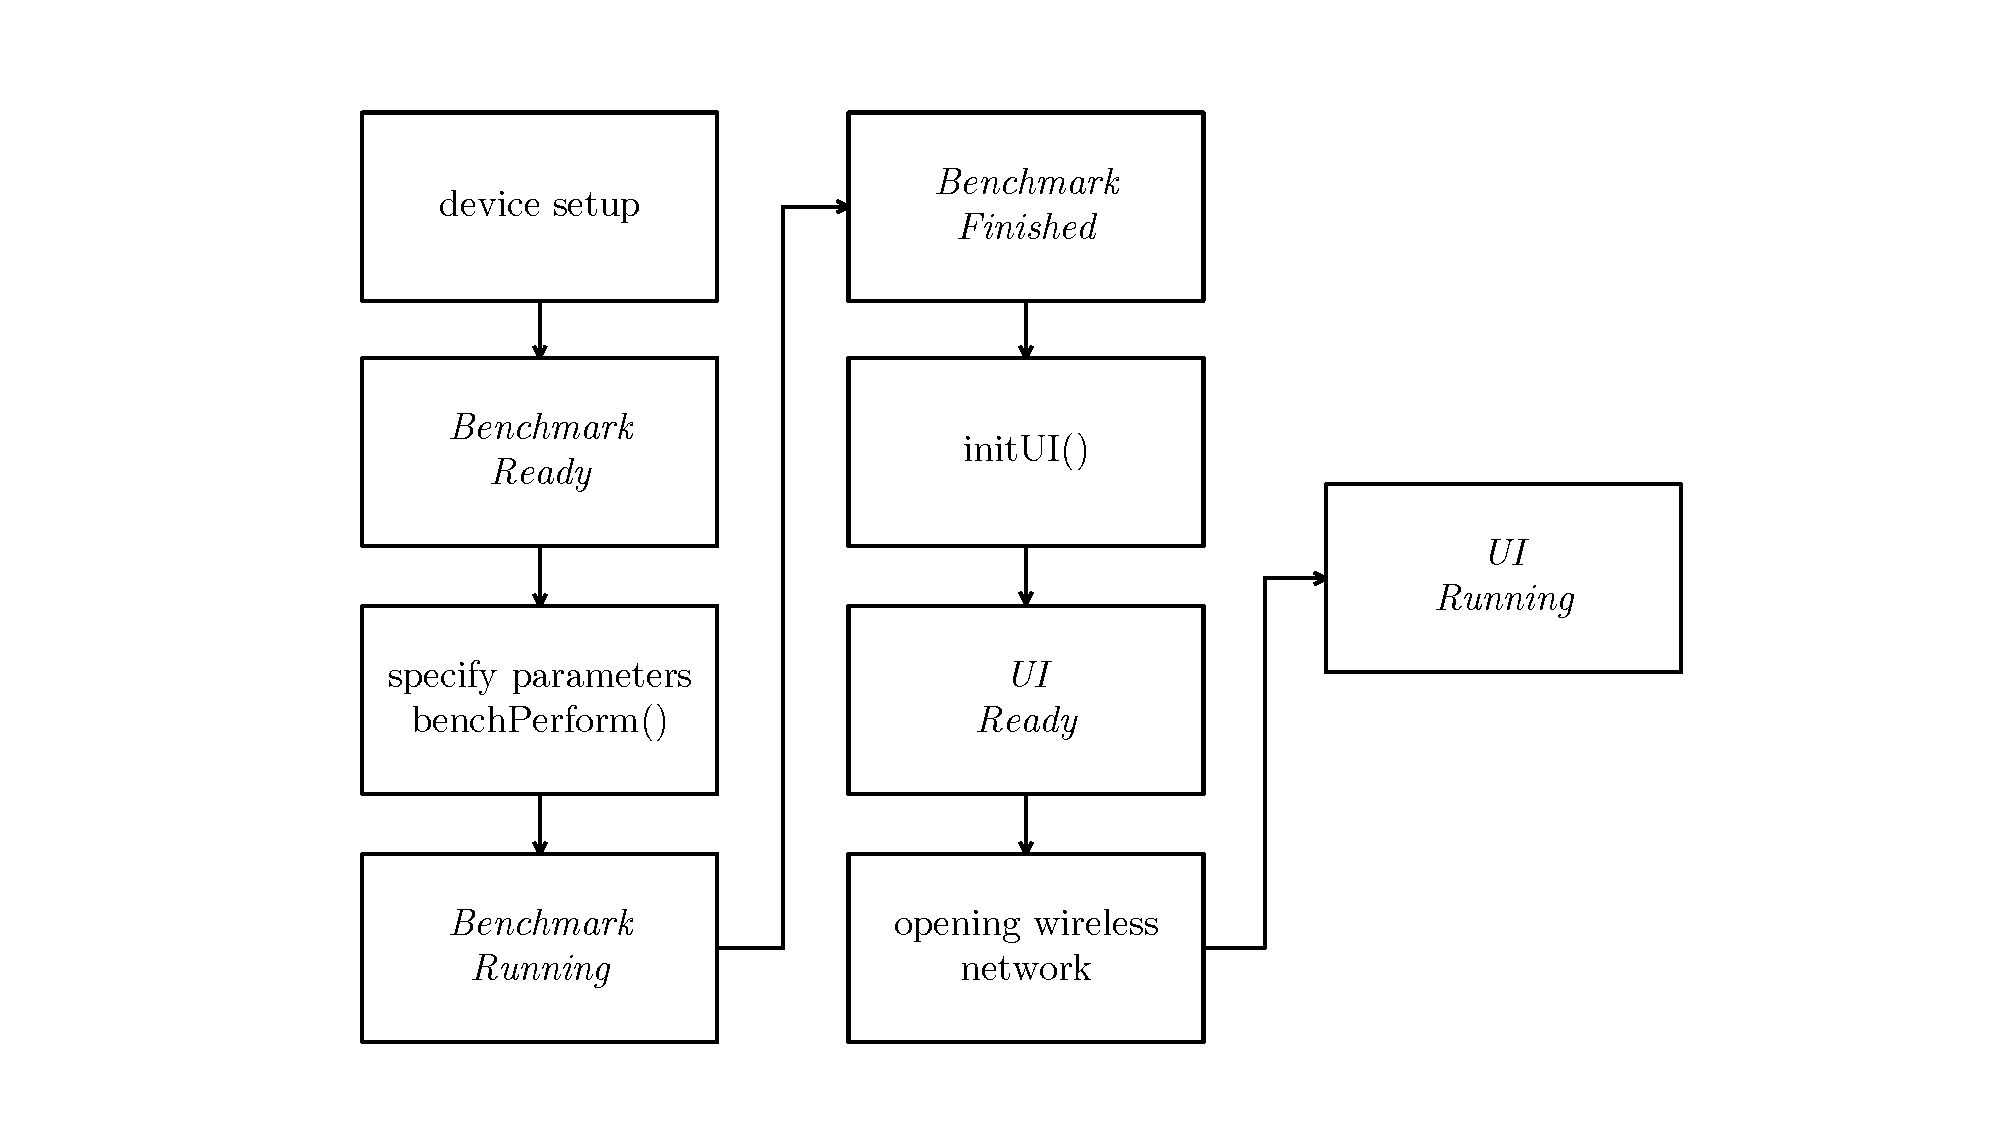
\includegraphics[width=1.1\linewidth]{images/State-Machine.pdf}}
	\caption{ State machine implementation for handling the UI, Benchmark stages }
	\label{fig:stateMachine}
\end{figure}  

Each state has its own set of parameters and will only switching the context to the next one if everything went fine. This is for preventing user errors by passing wrong arguments and to reduce runtime crashes. Nevertheless its also necessary because the UI needs several running threads in th background as well and this would lower the overall performance of the \textit{ESP32}, which we actually need for the \text{Benchmark}. So the UI is only allow to start after the results are calculated and saved correctly.\\   

\noindent The next chapter will now focus on the details of the C++ implementation of the \textit{Benchmark} for performing the Mandelbrot computation [see Chapter \ref{subsection:subImages}]. Beside that, we will describe the \textit{frontend} written in \textit{javascript}, especially the communication and data processing part [see Chapter \ref{subsection:frontend}]. 

\newpage

\subsection{Mechanism to divide the picture into sub areas} \label{subsection:subImages}

If now want to compute the Mandelbrot set, as we already describe in Chapter \ref{chap:mandelbrotIntroduction}, there are two possibilities to achieve this aim. And it definitely depends on the degree of complexity, which one we will choose. But first, let us describe the two main ways on how to compute the Mandelbrot set in parallel. 

Our aim is to split the image into sub sections, as we did the same for the part sums computation. What probably comes first in our mind is to split the Mandelbrot image using a division like a chess board [see Figure \ref{fig:mandelbrotChessboard}].

\begin{figure}[htbp]
	\centerline{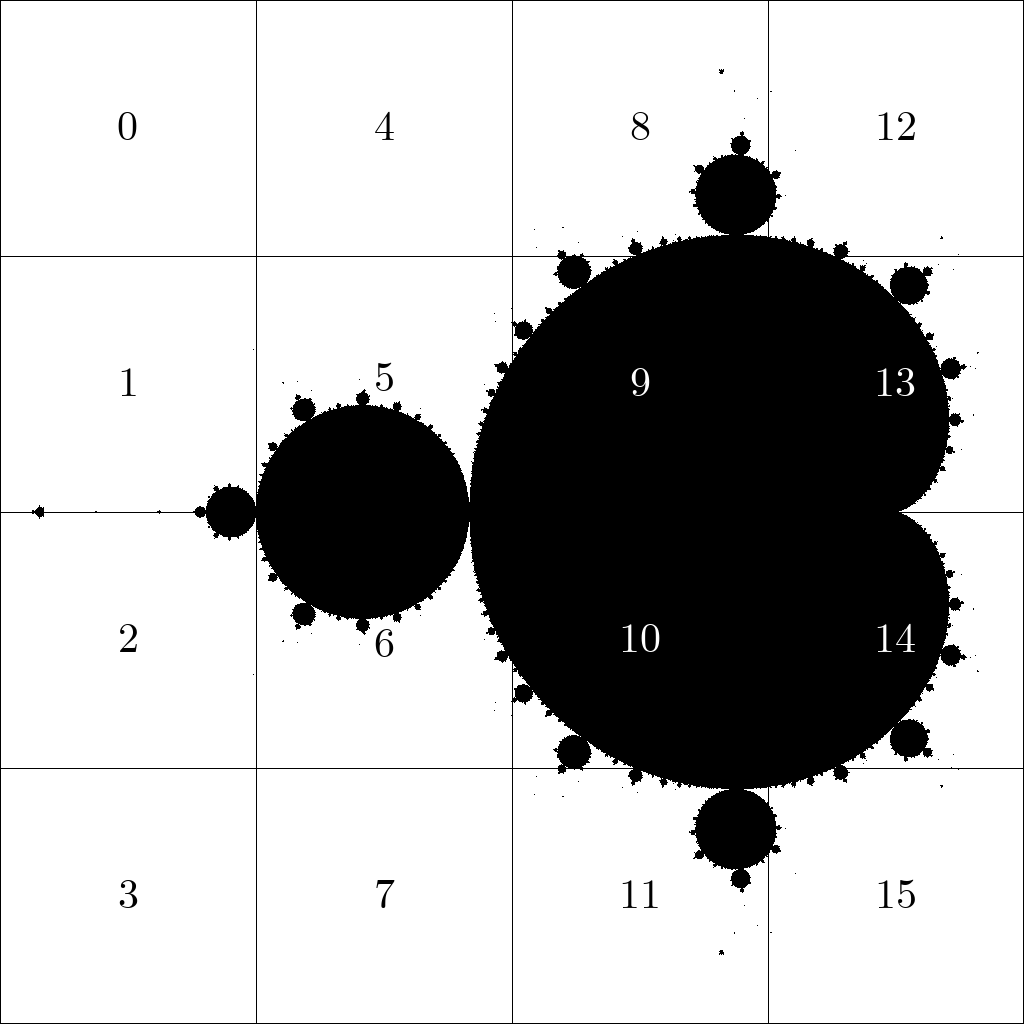
\includegraphics[width=0.75\linewidth]{images/mandelbrot-chess-board.png}}
	\caption{ Split the Mandelbrot image using the chess board method. }
	\label{fig:mandelbrotChessboard}
\end{figure} 

Each sub image is defined based on its start and end point from where its located. If we assume a resolution of 600 by 600 pixel, sub image number 5 would have its start point at P\textsubscript{5\textsubscript{Start}} (150, 150) and its end point at P\textsubscript{5\textsubscript{End}} (300, 300). Our Mandelbrot function, which has to calculate the Mandelbrot set, should receive beside the main image resolution the boundaries of the sub areas, which have to be calculated dynamically as well, so in this case the user has only to specify the number of part images, which corresponds to the amount of parallel threads. The possible number of sub images are limited on two facts: for the chess board method the passed value for the number of sub images has to be a even square root and of course, the division of width or height with the root of the passed value has to result in a even number as well. Those two case have to be catch in the computation function of the Mandelbrot set.

\newpage

\noindent Another method to split the image into sub areas would be using only rows. Each thread now has to calculate a part image with a resolution of width and height divided by the number of used threads. If want to split the work balanced regarding to the threads, its only allowed to specify an amount of threads which results in a even division of the height and this value. 

\begin{figure}[htbp]
	\centerline{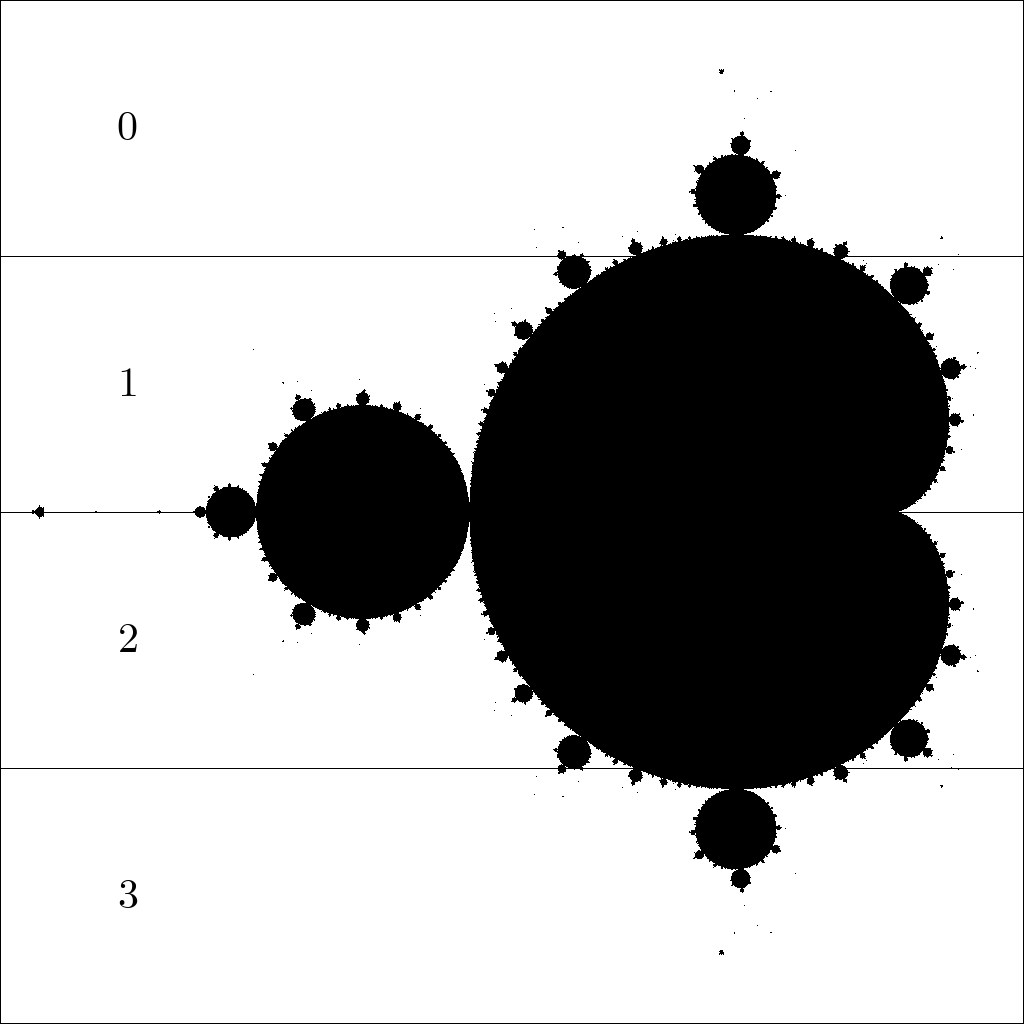
\includegraphics[width=0.75\linewidth]{images/mandelbrot-row.png}}
	\caption{ Split the Mandelbrot image using the row method. }
	\label{fig:mandelbrotRows}
\end{figure} 

To implement it more dynamically, we can assume also odd part images regarding to the height of the sub areas.
In this case, the last row would have a smaller height. E.g for a main image with a resolution of 600 by 600 pixel, the rows would have a dimension of 600 by 85 pixel for seven threads, the last one in fact only 600 by 5 pixel. 

A possible implementation for this scenario is seen in the following code snippet on the next page [see \ref{code:MandelbrotRow}]. Regarding to the specified parameters \textit{width}, \textit{height} and the amount of threads, the start and end points are computed very similar im comparison to the chess board method. But due to the fact that we have a fixed width, our x coordinates are fixed too. So we only have to compute the start and end y coordinate for each sub area. In case of a odd result of the number of threads and the specified height, we have to add the rest of that division for the last end point y coordinate.

\newpage

\begin{lstlisting}[label={code:MandelbrotRow}]
float Benchmark::runMandelbrotWith(unsigned int width, unsigned int height, int numThread) {
	
	...
	
	for (int j = 0; j < numThread; j++) {	
		unsigned minX = 0;
		unsigned maxX = width;
		unsigned minY = j * (height / numThread);
		unsigned maxY = (j+1) * (height / numThread);
		
		if(height % numThread != 0 && j == numThread - 1) {
			maxY += (height % numThread);
		}
		
		m[j] = new Mandelbrot(width, height, minX, maxX, 
								     minY, maxY, *queue);
		
		...

	}
}
\end{lstlisting}

The mechanisms to benchmark this kind of computation are similar to the sum example [see Chapter \ref{chap:simpleMathCompParallel}]. A time measurement has to be implemented as well as a \textbf{Message Passing Model} to signal the end of the computation of every thread. After that the part results have to be collected to save them as a \textit{*.ppm} image file [see Chapter \ref{subsection:ppm}].\\

\noindent Before we describe the image format we store the Mandelbrot set into, we go into further details about calculating the Mandelbrot set. As already described in Chapter \ref{chap:mandelbrotIntroduction}, the Mandelbrot set is based on a complex series defined by a simple function. Complex numbers are in fact 2-dimensional and they have an imaginary and real part. So in order to produce an image based on the complex series, we only have to plot the real part as x, the imaginary part as y coordinates on a 2D Cartesian system. If the calculated complex value belong to the Mandelbrot set, we will color this point red, otherwise black.

To get colors, we will use simple \textit{RGB} values, so therefore each color can be created with mixing the three primary colors red, green and blue. To simplify the whole process, we will only limit ourselves as mentioned above to the colors red and black. And we will not implement gradations in the colors. So basically, for red we will save a one, and for black a zero. But how is it possible to generate a printable image based on the result matrix, where the point information are stored? For this we will use image format called \textit{PPM}, the short form for ``\textit{portable pixmap format}'' [see Chapter \ref{subsection:ppm}].

\newpage

\subsection{Image file format ppm} \label{subsection:ppm}

A \textit{PPM} image is a uncompressed image file format in which the raw information of each pixel point is stored as a \textit{RGB} value. The header section of the file will contain the width and the height as well as maximum color number, for a gradient color value range 255, for only two possible states zero or one.

\begin{lstlisting}[caption=Simple example for an ppm image file format]
 P3				# ppm image format
 3 3			# width x height
 1				# maximum color value (0-255 or 1), val(r,g,b)

 0 0 0	=> black				-
 0 0 1	=> blue					|	first row
 0 1 0	=> green				-
 0 1 1	=> magenta				-
 1 0 0	=> red					|	second row
 1 0 1	=> turquoise			-
 1 1 0	=> yellow				-
 1 1 1	=> white				|	third row
 0 0 0 							-
\end{lstlisting}

This will basically create a pixel matrix of three by three pixel filled with primary colors like shown in figure underneath.

\begin{figure}[htbp]
	\centering
	\begin{subfigure}{.5\textwidth}
			\centerline{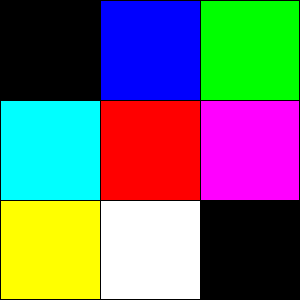
\includegraphics[width=0.75\linewidth]{images/ppm.png}}
			\label{fig:pixelPPMColors}
	\end{subfigure}%
	\begin{subfigure}{.5\textwidth}
		\centerline{
\includegraphics[width=0.75\linewidth]{images/ppm-2.png}}
		\label{fig:pixelPPMSimplified}
	\end{subfigure}
	\caption{Colored and limited example of a simple pixel matrix image.}
	\label{fig:pixelPPM}
\end{figure}

\noindent To interpret the \textit{PPM} image file, we will read the header information, extract the width and height to go through the underneath stored \textit{RGB} values. Each value will represent one pixel color and if a row is finished, a new starts; The pixel colors are simply listed one after the other. 

If we now simplify that to the mentioned colors red and black, we would create a image only based on these colors. This is exactly what we are do when we compute the Mandelbrot set, and if we find a point which is inside the Mandelbrot set M, we assign a color, otherwise we will leave this point black.

\newpage

\subsection{Compression for reducing file size}

So far, we haven't discussed the advantages or disadvantages of both methods to split the Mandelbrot image into sub areas mentioned in Chapter \ref{subsection:subImages} and which one we will finally choose. Both methods are perfectly implementable on a machine with enough memory resources, especially \textit{RAM} and \textit{flash memory}. But if we think about our micro controller, the \textit{ESP32}, we have indeed limited resources. So calculating and saving the Mandelbrot set on the \textit{ESP32} is kind of different than on a usual x86 architecture with for example a powerful i7 processor in combination with 8GB of \textit{RAM}.  

If we want to have a precisely computation of the Mandelbrot image, it is necessary to have a quite high resolution, the colors for the sections inside or outside of the Mandelbrot set are not that important, to reduce file size, we limit them to red and black, because basically the \textit{ppm} image is nothing more than a text file, so every character we save will decrease the file size.

\begin{lstlisting}[caption=Reduced ppm image file format, label=list:ppmReduced]
 P3				# ppm image format
 600 600		# width x height
 1				# maximum color value
 
 0
 0
 1
 1
 0
 1
 0
 1
\end{lstlisting}

For an image with a resolution of 600 by 600 pixel we have 360000 characters to save including the header section and the carriage return line feed character for each new line. This will result in an overall file size of 2.2MB regardless of the pixel color information itself. The question arise if there is still a way to decrease the amount of characters we have to store. If we take a closer look to the example file above [see Listing \ref{list:ppmReduced}], the information containing the Mandelbrot set is actually a bit stream, so what happen if combine a specific amount of those bits to a new value, probably one who has less characters overall.

\begin{figure}[htbp]
	\centerline{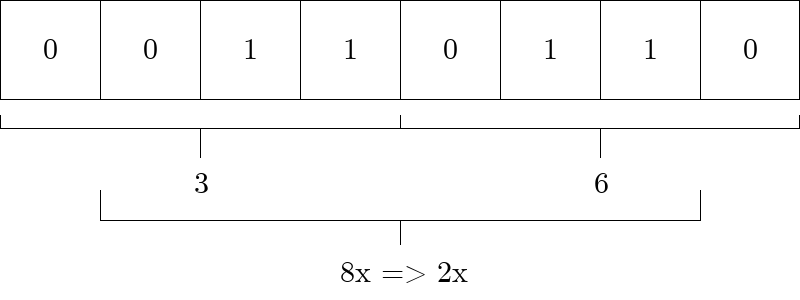
\includegraphics[width=0.75\linewidth]{images/compression-2.png}}
	\caption{ Method to reduce characters in a \textit{PPM} file. }
	\label{fig:ppmCompression}
\end{figure} 

\newpage

The procedure is quite simple: we just collect a specific amount of values - we will call them bits, in fact, they are true characters - and we interpret them as bits so that we can create based on these combinations a new real Integer value. A possible scenario is shown in Figure \ref{fig:ppmCompression} were we combine each 4 bits to a new Integer value.\\

\noindent The question now could be how many bits we can possible combine? What are our limits? Well, first of all let's think in block buffers: If we have the first line of our Mandelbrot image, for a resolution of 600 by 600 pixel, we have 600 bits defining our first pixel row. To start a combining process, we have to check whether its possible to split those 600 bits into an even number of block buffers. So let's say into 120, that would mean we combine every 5 bits, because 600 divided by 120 result in 5. All odd number of block buffers are forbidden; this scenario i think is quite comprehensibly. Now its time to take into account both methods on how to split the Mandelbrot image into sub areas. However, we want to keep the compression and decompression process as simple as possible, that means only the last method is capable of achieving this aim, because using the first method, we have to be very carefully by combining the compressed part results to the final image; each compressed line form one part image belongs to several other lines on the same row.

\begin{center} \label{graph:fileCompression}
	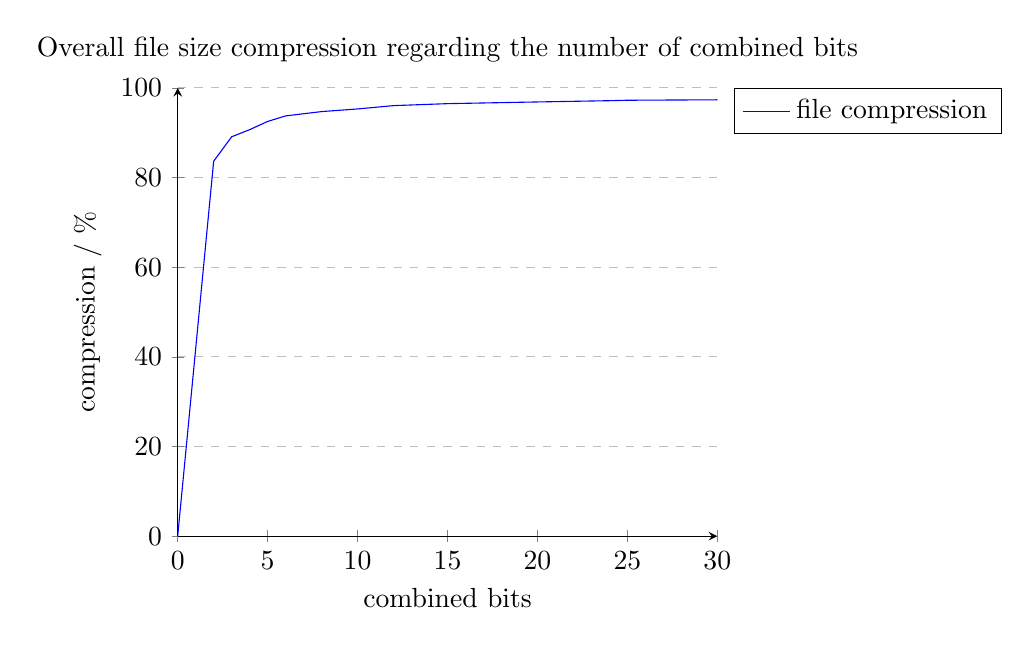
\begin{tikzpicture}
	\begin{axis}[
	 	title={Overall file size compression regarding the number of combined bits},
		axis lines = left,
		xlabel = {combined bits},
		ylabel = {compression / \%},
		xmin=0, xmax=30,
		ymin=0, ymax=100,
		legend pos=outer north east,
		ymajorgrids=true,
		grid style=dashed,
	]
	\addplot [
		domain=0:30, 
		samples=10, 
		color=blue,
	]
	coordinates {
		(0,0)(2, 83.64)(3, 89.09)(4, 90.68)(5, 92.51)(6, 93.75)(8, 94.71)(10, 95.3)
		(12, 96.04)(15, 96.48)(20, 96.86)(24, 97.14)(25, 97.24)(30, 97.34)
	};
	\addlegendentry{file compression}
	
	\end{axis}
	\end{tikzpicture}
\end{center}

Back to our combining problem: So how many bits can we combine as a maximum amount? We are literally limited to the hardware we are using. Based on the fact that we cast our bit stream to an Integer value, the maximum bits an Integer value can store depends on our hardware platform. For a 32-bit architecture, which also includes the \textit{ESP32}, we have 32-bits for an Integer value. 

Build on these facts, we are able to plot a graph which shows the relation between the result file size and the number of combined bits [see Graph \ref{graph:fileCompression}].\\

\noindent We have to keep in mind that the number of combined bits depends on the specified resolution of the Mandelbrot image. Also, this method is not optimized in case of execution time, because the main bottle neck was storing the result into the \textit{flash memory} and reducing \textit{bandwidth} for transmitting the final result image to the webfrontend. 

\newpage

\subsection{Graphical visualization} \label{subsection:frontend}

Our results we will receive from the \textit{Benchmark} class are first of all the execution time values regarding how many threads we used to compute the problem in parallel (the \textit{Computation.h} or the \textit{Mandelbrot.h}), and of course, the Mandelbrot set as a \textit{ppm} image.

A way to present those results state of the art is a visualization without any additional software which the user has to install. So we decided to implement a webfrontend, which can be easily accessed from the \textit{ESP32} itself through logging into the created wireless network and opening the users web browser. The web page is written in \textit{VueJS}, a \textit{Javascript} framework, and uses asynchronous \textit{http} requests and a websocket connection to communicate with the \textit{ESP32} \textit{backend}.

\begin{figure}[htbp]
	\centerline{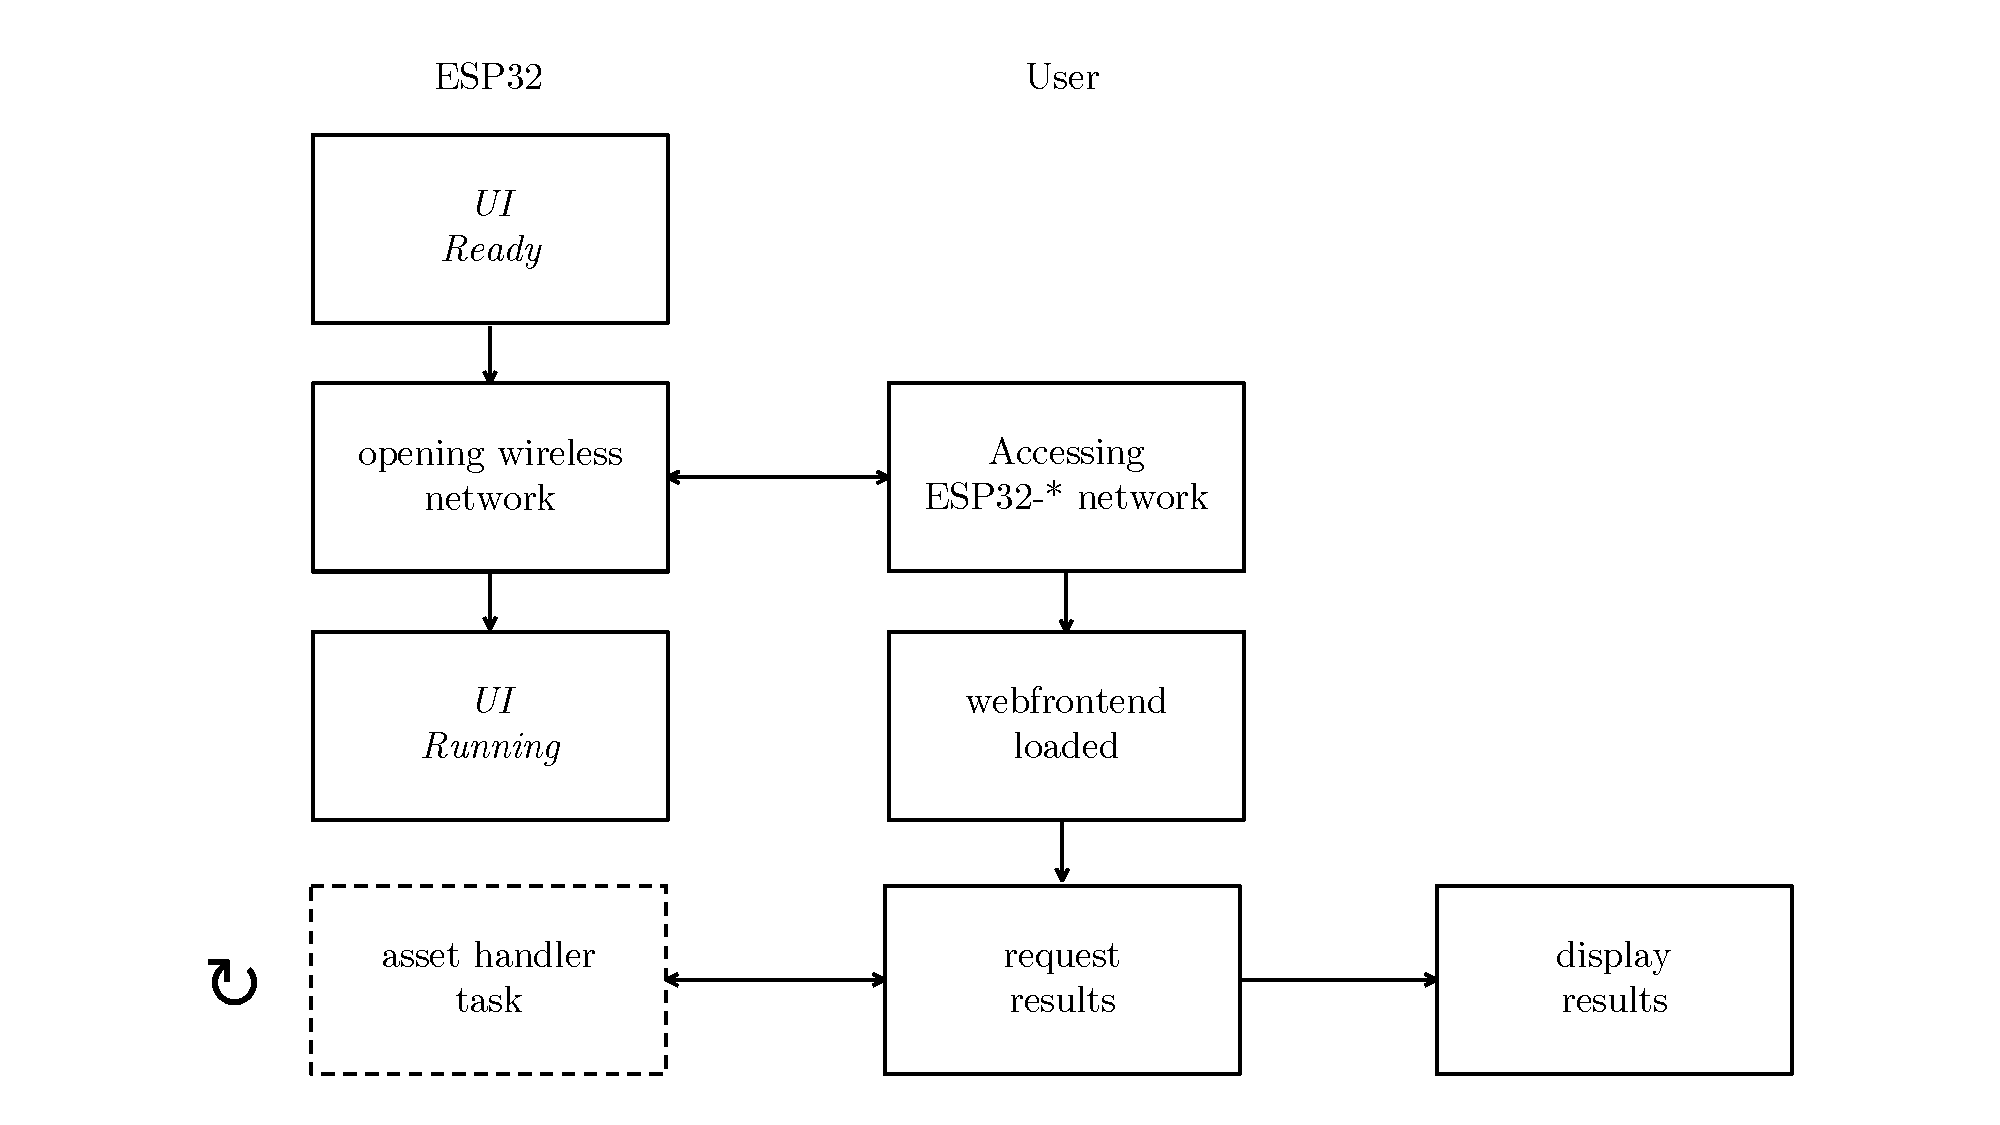
\includegraphics[width=1.1\linewidth]{images/State-Machine-Webforntend.pdf}}
	\caption{ State machine implementation for frontend-backend communication. }
	\label{fig:stateMachineWebfrontend}
\end{figure}  

The main part for the \textit{frontend} is basically to decompress the received \textit{ppm} image file and to plot the execution time results taken from the benchmark for the \textit{Computation} and \textit{Mandelbrot} example. Between the \textit{frontend} and the \textit{backend}, the number of combined bits are preset, because we are trying to combine as a maximum 30 bits regarding to the specified width, so this number can be less than 30, but we try to combine as much as possible. This number has to be preset, otherwise the decompression will fail. The received \textit{ppm} image, after it is decompressed, will be printed on a canvas, so basically we loop through the \textit{ppm} image and set pixel by pixel regarding whether we have to give them a color or not.\\

\noindent For displaying the execution time results, we use \textit{ChartJS}, an additional component to plot charts with \textit{Javascript}. We use four charts to display the execution time of both examples as well as the gained speed up factor. But we will only transmit to the \textit{frontend} the execution time values, because the speed up factors can be calculated on \textit{frontend} side to reduce bandwidth.

\newpage

\section{Benchmark setup of the Mandelbrot fractal computation} \label{chap:benchmarkSetup}

Now we will take into account how to finally start the whole benchmark process. This will include initializing the necessary parameters for the \textit{Computation} and \textit{Mandelbrot} example and how to enable the \textit{frontend} to display the results graphically.

At First, we have to include the \textit{BemchmarkHandler.h} class. This class will include the \textit{Benchmark.h} file and serve all necessary functions to start and to handle the different states of the benchmark process. Due to the fact that we are using several threads for different task, we decided to have at least to global pointers to ensure access to the necessary resources. To avoid race conditions, most of the functions are covered with \textit{Mutex's}, or are it was ensured that the function will only be accessed from one thread. 

\begin{lstlisting}[label=list:benchmarkHandler, caption=Necessary include's for the benchmark setup]
#include "libs/benchmark/BenchmarkHandler.h"
#include "libs/websocket/WebsocketHandler.h"

BenchmarkHandler *handler;
WebsocketHandler *wsHandler;

void setup() {
	/* serial communication */
	Serial.begin(115200);
	
	/* initialize internal storage */
	if(!SPIFFS.begin(true)){
		Serial.println("[main] SPIFFS mount failed.");
		return;
	}
	
	delay(1000);
	
	...
	
}
\end{lstlisting}

After defining the global pointers, we will initialize the \textit{uart} interface to enable serial communication for debug purposes and the internal \textit{flash memory} for saving our results to files. To start on of our benchmark examples, we have to call the related callback functions:

\begin{lstlisting}[label=list:benchmarkHandlerStart, caption=Example on how to start the benchmark process]
	handler = new BenchmarkHandler(16);

	handler->startComputationBenchmark();
	handler->startMandelbrotBenchmark();
\end{lstlisting}

\newpage

By setting up the object on the \textit{heap} by calling the \textit{new} operator, we pass through the constructor the amount of threads we want to create regardless which benchmark example we will execute, so this number of threads will be fixed.

Every time we start a benchmark example, the execution time results will be stored in the handler's properties. To display them, we have to call \textit{displayResult()} method. In fact, the results are also stored after each benchmark run in a local \textit{results.txt} file in the internal \textit{flash memory}. The first line of the file will contain the results of the first run of the benchmark, the second one the ones of the second run of the benchmark.

\begin{lstlisting}[label=list:benchmarkHandlerStart, caption=The final benchmark code.]
void setup() {
	...
	
	handler = new BenchmarkHandler(16);
	
	/* first we run the Computation example */	
	handler->startComputationBenchmark();
	handler->displayResult();
	
	/* The Mandelbrot fractal will be stored in mandelbrot.ppm */
	handler->startMandelbrotBenchmark();
	handler->displayResult();
	
	handler->finalize();
}
	
void loop() {
	handler->displayUI();
}
\end{lstlisting}

If the benchmark runs finished successfully, we are able to finalize the process by calling the method \textit{finalize()}. This method will check whether all results are stored and benchmark finished successfully. Only in this case, it will enable the \textit{UI\_Ready} state, so the \textit{ESP32} can create a wireless network and serve the necessary web files for the \textit{frontend}.

Meanwhile, the infinite main loop while wait until the UI state changed to \textit{UI\_RUNNING}, after that the user is able to access the results from the \textit{frontend} loaded in the users web browser.

\chapter{Conclusion}\label{chap:conclusion}
After running the benchmark functions mentioned in Chapter \ref{chap:benchmarkSetup}, the \textit{ESP32} will serve a wireless network, on which the user can log into. While entering the default IP address (\textit{192.168.4.1}) of the \textit{ESP32}, the \textit{backend} will serve all web files. 

\begin{figure}[htbp]
	\centerline{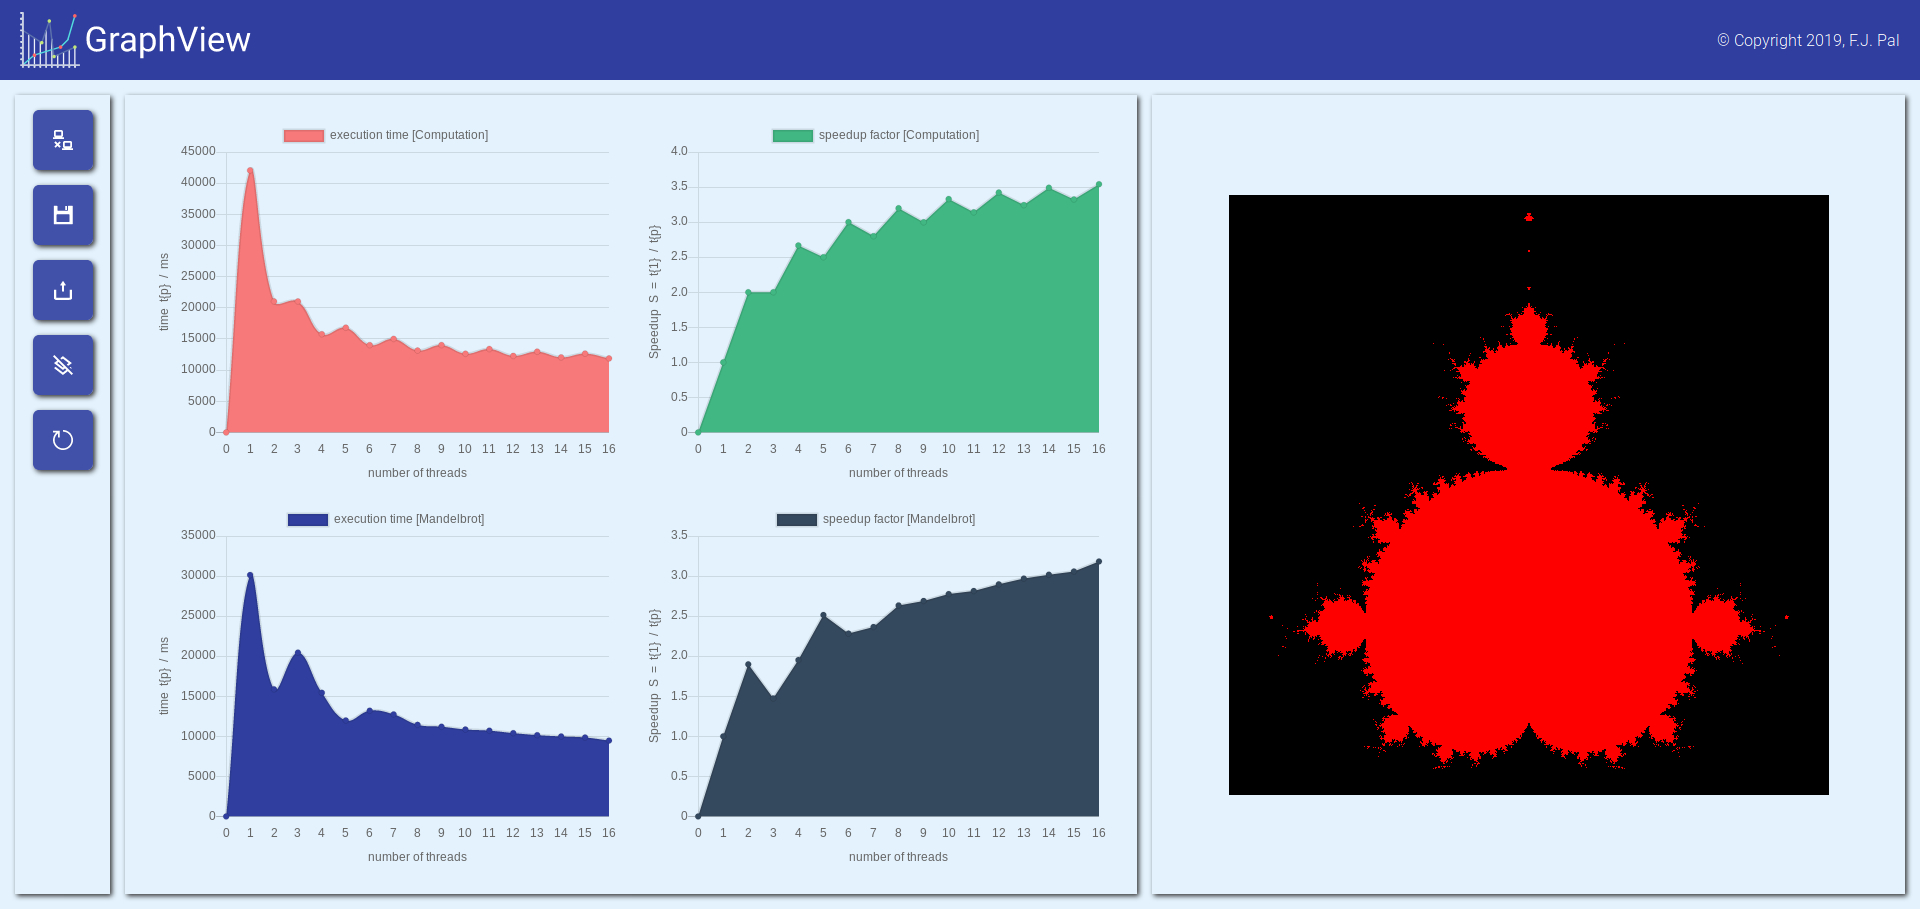
\includegraphics[width=0.95\linewidth]{images/demo.jpg}}
	\caption{ Successfully loaded \textit{frontend} with all results. }
	\label{fig:frontendResults}
\end{figure}  

The calculated results can now be loaded to the \textit{frontend} using the buttons on the left. Therefore it is necessary to open the websocket connection to the \textit{ESP32} (first button). After that we can proceed with downloading the results to our local drive by using the save button.

For both examples the chart results are quite impressive. Even after we left real time parallelism (limited to the real number of cores on the hardware system), in our case two threads running independently on different cores, it was possible to achieve a speedup. By using 62 threads for both examples, we were able to reach a maximum number of speed up of 3.65 (\textit{Mandelbrot}) and 3.7 (\textit{Computation}). Due to the fact that we run the \textit{Benchmark} on a real time operating system (\textit{FreeRTOS}), several runs of the same setup will result into almost the same results regarding execution time, because the execution time of each instruction is predictable.

The charts mentioned on the next page leads us to the assumption, that for our setup we will reach some kind of limit in speedup. But its not really comparable to the limit Amdahl's Law predicted, because we are not using real processor cores, we are dealing with thread level parallelism.

\newpage

\begin{figure}[htbp]
	\centerline{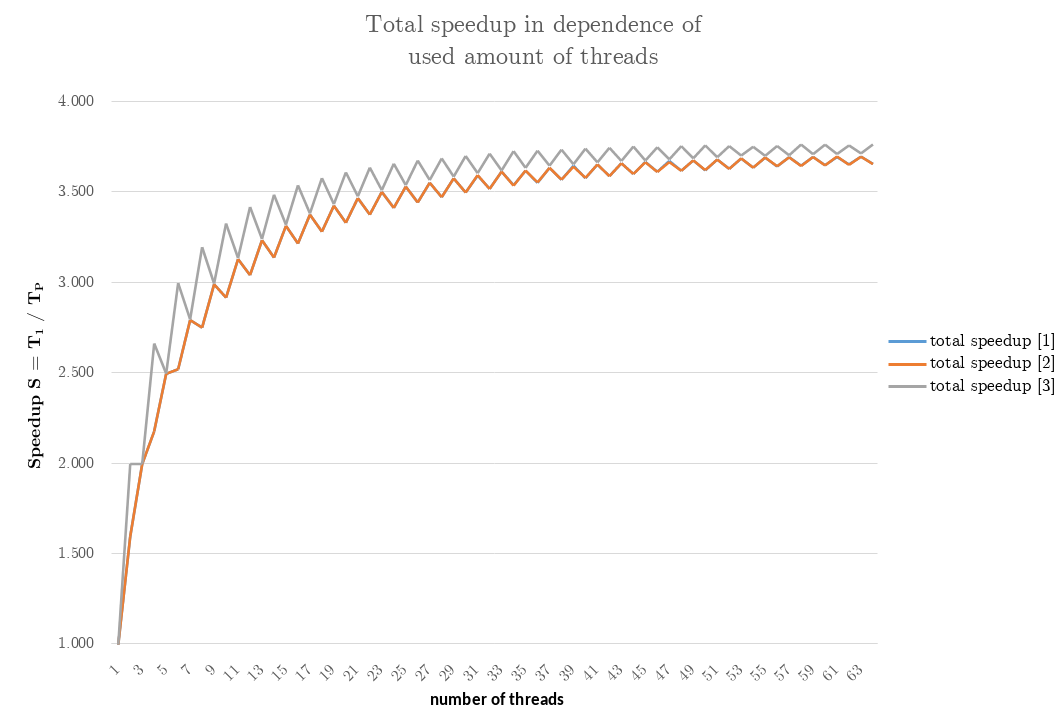
\includegraphics[width=0.8\linewidth]{images/evaluation-computation.png}}
	\caption{ Speedup factor gain for the \textit{Computation} example. }
	\label{fig:resultsComputation}
\end{figure}  

\begin{figure}[htbp]
	\centerline{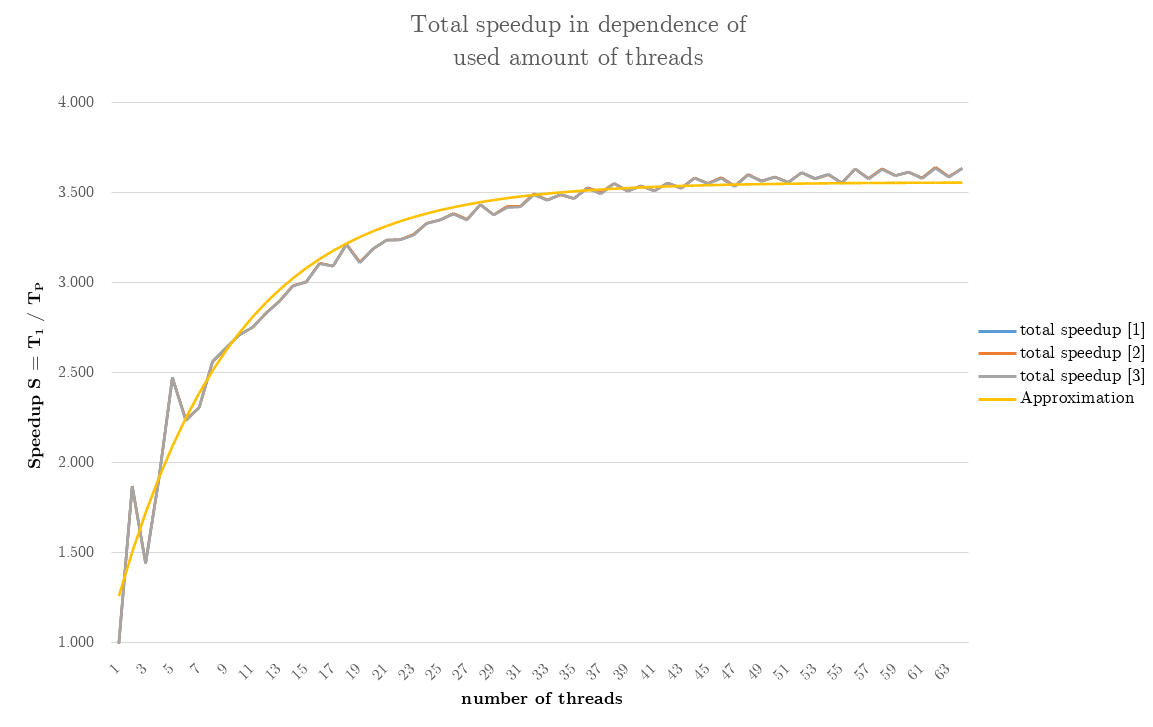
\includegraphics[width=0.8\linewidth]{images/evaluation-mandelbrot.png}}
	\caption{ Speedup factor gain for the \textit{Mandelbrot} example. }
	\label{fig:resultsMandelbrot}
\end{figure}  

\printbibliography
%\nocite{*}

\end{document}